\chapter{HASIL DAN PEMBAHASAN} \label{Bab IV}

\section{Hasil Penelitian} \label{IV.Hasil}
Bagian ini menyajikan hasil penelitian yang diperoleh dari seluruh tahapan yang telah dilakukan. Proses penelitian meliputi ekstraksi dan analisis data SSGI tahun 2024 pada tingkat provinsi, dilanjutkan dengan tahap pra-pemrosesan data hingga pembangunan model prediktif. Model yang digunakan dalam penelitian ini adalah \textit{Random Forest} untuk memprediksi prevalensi \textit{stunting}, yang kemudian dikombinasikan dengan metode \textit{SHAP} untuk menjelaskan kontribusi masing-masing variabel. Seluruh proses pemodelan dilakukan menggunakan skema validasi LOOCV serta optimasi parameter melalui \textit{GridSearchCV} untuk memperoleh kinerja model yang optimal.

\subsection{Analisis Deskriptif}
Penelitian ini menggunakan data sekunder yang berasal dari laporan resmi SSGI tahun 2024 yang dipublikasikan oleh Badan Kebijakan Pembangunan Kesehatan (BKPK) Kementerian Kesehatan RI. Data pada bentuk aslinya berupa rekapitulasi persentase berbagai indikator kesehatan, gizi, dan sosiodemografi yang tersebar dalam beberapa bagian laporan. Karena penelitian ini menggunakan pendekatan \textit{machine learning} berbasis data tabular, format tersebut tidak dapat langsung digunakan sehingga diperlukan proses ekstraksi dan penyusunan ulang data. Proses ekstraksi dilakukan dengan memilih indikator yang relevan dan menyusunnya ke dalam bentuk tabel dengan baris dan kolom yang terstruktur. Hasilnya, data dibagi menjadi satu variabel target yaitu prevalensi \textit{stunting} serta sejumlah variabel prediktor yang mencerminkan faktor-faktor seperti sanitasi, pola asuh, dan pendidikan ibu.

\textit{Dataset} akhir yang digunakan dalam penelitian ini terdiri dari 36 baris observasi yang mewakili provinsi di Indonesia. Setiap baris tersebut memuat nilai persentase dari variabel target dan variabel prediktor yang telah disusun dalam format seragam. Penyusunan bentuk tabular ini bertujuan agar matriks data dapat langsung diolah pada tahapan komputasi menggunakan algoritma \textit{machine learning}. Selain itu, format terstruktur ini memudahkan jalannya tahapan pra-pemrosesan dan seleksi fitur sebelum model dibangun. Kumpulan data final sejumlah 36 provinsi inilah yang menjadi dasar utama dalam proses pelatihan serta evaluasi sistem.

\subsection{Persiapan Data}
Laporan SSGI tahun 2024 disajikan dalam bentuk dokumen \textit{Portable Document Format} (PDF) yang memuat sekitar 5.189 tabel statistik yang berisi berbagai indikator kesehatan, gizi, serta kondisi sosial dan lingkungan. Data dalam laporan tersebut mencakup informasi terkait kesehatan ibu dan anak, pola asuh, akses layanan kesehatan, sanitasi, serta karakteristik demografi rumah tangga dengan fokus pada balita usia 0--59 bulan menggunakan pendekatan \textit{cross-sectional}. Meskipun data tersedia pada beberapa tingkat wilayah seperti nasional, provinsi, dan kabupaten/kota, penelitian ini hanya menggunakan tingkat provinsi sebagai unit analisis untuk melihat perbedaan determinan \textit{stunting} secara umum. Struktur data dalam bentuk laporan ini belum dapat langsung digunakan untuk pemodelan \textit{machine learning}, sehingga diperlukan proses pengolahan lebih lanjut. Oleh karena itu, kondisi awal dan karakteristik data sebelum dilakukan ekstraksi disajikan pada Tabel \ref{table:4.kondisi_awal}.

\begin{longtable}{|c|p{0.3\textwidth}|p{0.5\textwidth}|}
    \caption{Kondisi Awal Dataset SSGI 2024}
    \label{table:4.kondisi_awal}\\
    \hline
    \textbf{No} & \centering\textbf{Atribut} & \textbf{Keterangan Kondisi Awal} \\ 
    \hline
    \endfirsthead
    \hline
    \textbf{No} & \centering\textbf{Atribut} & \textbf{Keterangan Kondisi Awal} \\ 
    \hline
    \endhead
    \hline
    1 & Sumber / Penerbit Data & Badan Kebijakan Pembangunan Kesehatan (BKPK) Kementerian Kesehatan RI \\
    \hline
    2 & Format File & Dokumen Laporan \textit{Portable Document Format} (PDF) \\ 
    \hline
    3 & Volume Data & $\pm$ 5.189 tabel statistik \\
    \hline
    4 & Variabel Target (\textit{Label}) & Angka prevalensi balita \textit{stunted} (pendek) berdasarkan indeks Tinggi Badan menurut Umur (TB/U) \\
    \hline
    5 & Cakupan Indikator (\textit{Fitur}) & Kesehatan ibu dan anak, pola asuh, akses kesehatan, sanitasi, dan sosiodemografi \\
    \hline
    6 & Populasi Target & Rumah tangga kelompok balita usia 0-59 bulan \\
    \hline
    7 & Tingkat Agregasi Wilayah & Nasional, Provinsi (38 Provinsi), dan Kabupaten/Kota \\
    \hline
    8 & Pendekatan Pengambilan & \textit{Cross-sectional} (Satu titik waktu tertentu) \\
    \hline
    9 & Format Nilai Data & Numerik dan Persentase (\%) \\
    \hline
\end{longtable}

\subsubsection{Ekstraksi Data}
Tahap ekstraksi data dilakukan untuk memindahkan informasi prevalensi dan indikator kesehatan dari dokumen PDF SSGI 2024 ke dalam bentuk data yang lebih terstruktur. Proses ini menggunakan fitur \textit{Power Query} pada Microsoft Excel yang mampu membaca dan mengimpor tabel secara otomatis dari dokumen. Setelah seluruh tabel berhasil diambil, dilakukan penyaringan untuk memilih tabel yang sesuai dengan kebutuhan penelitian, khususnya yang memuat data tingkat provinsi dan indikator determinan \textit{stunting}. Setiap tabel yang dipilih kemudian diperiksa kembali dengan sumber aslinya untuk memastikan tidak terjadi kesalahan posisi data. Hasil dari tahap ini berupa kumpulan tabel mentah yang siap digunakan pada proses selanjutnya, yang dapat dilihat pada Tabel \ref{table:4.hasil_ekstraksi}.

\begin{longtable}{|c|c|p{0.55\textwidth}|}
    \caption{Contoh Hasil Ekstraksi Tabel dari Laporan SSGI 2024}
    \label{table:4.hasil_ekstraksi}\\
    \hline
    \textbf{No} & \textbf{Nomor Tabel Laporan} & \textbf{Indikator yang Diekstrak} \\ 
    \hline
    \endfirsthead
    \hline
    \textbf{No} & \textbf{Nomor Tabel Laporan} & \textbf{Indikator yang Diekstrak} \\ 
    \hline
    \endhead
    \hline
    \endfoot
    \hline
    \endlastfoot
    1 & Tabel 4.3 & Status Gizi Tinggi Badan menurut Umur (TB/U) \\ 
    \hline
    2 & Tabel 5.15 & Pemeriksaan Kehamilan Ibu \\
    \hline
    3 & Tabel 5.33 & Pemberian ASI Eksklusif 6 Bulan \\
    \hline
    4 & Tabel 5.113 & Status Imunisasi Dasar Balita (12-23 Bulan) \\
    \hline
    5 & Tabel 5.184 & Akses Sanitasi Rumah Tangga (RT) \\
    \hline
\end{longtable}

\subsubsection{Seleksi Fitur Determinan}
Tahap seleksi fitur dilakukan untuk menentukan variabel yang akan digunakan dalam pemodelan. Proses ini dilakukan dengan memilih indikator yang relevan berdasarkan kajian literatur dan pedoman resmi terkait determinan \textit{stunting}. Variabel yang dipilih mencakup beberapa aspek utama seperti prevalensi \textit{stunting}, kondisi sosial ekonomi, sanitasi, serta pola asuh dan pelayanan kesehatan. Sementara itu, indikator yang tidak berhubungan langsung dengan kondisi gizi balita tidak disertakan dalam analisis. Melalui proses ini, diperoleh kumpulan fitur yang dianggap paling mewakili kondisi tiap provinsi, sebagaimana disajikan pada Tabel \ref{tabel:4.seleksi_fitur}.

\begin{longtable}{|c|p{0.3\textwidth}|p{0.5\textwidth}|}
    \caption{Contoh Variabel Hasil Seleksi Fitur Determinan \textit{Stunting}}
    \label{tabel:4.seleksi_fitur}\\
    \hline
    \centering\textbf{No} & \centering\textbf{Aspek Determinan} & \textbf{Nama Variabel (Fitur Asli Laporan)} \\ 
    \hline
    \endfirsthead
    \hline
    \centering\textbf{No} & \centering\textbf{Aspek Determinan} & \textbf{Nama Variabel (Fitur Asli Laporan)} \\ 
    \hline
    \endhead
    \hline
    \endfoot
    \hline
    \endlastfoot
    1 & \textit{Outcome} (Target) & Prevalensi \textit{Stunting} (\%)\\ 
    \hline
    2 & Kondisi Fisik Lahir & Persentase Berat Badan Lahir Rendah (BBLR) \\
    \hline
    3 & Asupan Gizi Balita & Persentase Tidak Konsumsi Protein Hewani \\
    \hline
    4 & Penyakit Infeksi & Persentase Balita TBC \\
    \hline
    5 & Kapasitas Sosiodemografi & Persentase Pengetahuan \textit{Stunting} Baik \\
    \hline
\end{longtable}

\subsubsection{Transformasi dan Agregasi Data}
Tahap transformasi dan agregasi data merupakan proses penyatuan akhir sekaligus penyederhanaan struktur variabel agar memiliki makna dan skala yang konsisten saat dibandingkan antarprovinsi. Pada tahap ini, fitur yang telah diekstraksi digabungkan ke dalam satu matriks \textit{dataframe} menggunakan nama provinsi sebagai kunci penghubung (\textit{primary key}). Selain penggabungan tabel, dilakukan proses agregasi sistematis dengan mengombinasikan beberapa indikator yang memiliki kemiripan risiko, seperti menjumlahkan persentase kelompok usia kehamilan ekstrem menjadi satu atribut tunggal guna menghindari redundansi informasi. Seluruh variabel hasil agregasi tersebut tetap dipertahankan dalam satuan persentase untuk memastikan keseragaman format data sebelum diproses oleh algoritma pemodelan. Rincian mengenai sumber tabel laporan, alur operasi matematis yang diterapkan, hingga penamaan atribut baru yang masuk ke dalam \textit{dataset} utama dapat dilihat secara lengkap pada Tabel \ref{table:4.skenario_agregasi}.

\begin{longtable}{|c|p{0.18\textwidth}|p{0.38\textwidth}|p{0.22\textwidth}|}
    \caption{Contoh Skenario Transformasi dan Agregasi Fitur Determinan \textit{Stunting}}
    \label{table:4.skenario_agregasi}\\
    \hline
    \centering\textbf{No} & \centering\textbf{Nama Tabel Laporan} & \centering\textbf{Alur Sistematis \& Logika Agregasi} & \centering\textbf{Nama Atribut Baru (CSV)} \tabularnewline 
    \hline
    \endfirsthead
    \hline
    \centering\textbf{No} & \centering\textbf{Nama Tabel Laporan} & \centering\textbf{Alur Sistematis \& Logika Agregasi} & \centering\textbf{Nama Atribut Baru (CSV)} \tabularnewline 
    \hline
    \endhead
    \hline
    \endfoot
    \hline
    \endlastfoot
    
    1 & \raggedright Tabel 4.3 (Status Gizi TB/U) & \raggedright Menggabungkan persentase kategori \textit{Severely Stunting} dan \textit{Stunting} menjadi satu prevalensi target utama. & \texttt{prevalensi\_ stunting\_ persen} \tabularnewline 
    \hline
    
    2 & \raggedright Tabel 5.5 (Usia Ibu Memulai Kehamilan) & \raggedright Menjumlahkan dua persentase kategori usia ekstrem, yakni kelompok usia $<21$ tahun dan $>40$ tahun. & \texttt{persen\_ usia\_ ibu\_ berisiko} \tabularnewline
    \hline
    
    3 & \raggedright Tabel 5.184 (Akses Sanitasi RT) & \raggedright Menjumlahkan nilai dari kategori: BABS Terbuka, BABS Tertutup, dan Akses Belum Layak. & \texttt{persen\_ akses\_ sanitasi\_ berisiko} \tabularnewline
    \hline
    
    4 & \raggedright Tabel 5.33 (Pemberian ASI Eksklusif) & \raggedright Menghitung nilai komplemen (100\% dikurangi persentase "Hanya ASI 0-5 Bulan"). & \texttt{persen\_ tidak\_ asi\_ eksklusif} \tabularnewline
    \hline
    
    5 & \raggedright Tabel 5.113 (Status Imunisasi Dasar) & \raggedright Menggabungkan persentase balita dengan status imunisasi "Tidak Lengkap" dan "Tidak Imunisasi". & \texttt{persen\_ imunisasi\_ dasar\_ incomplete} \tabularnewline
    \hline
\end{longtable}


\subsection{Pra-pemrosesan dan Eksplorasi Data}
Tahapan pra-pemrosesan data bertujuan untuk mengubah \textit{dataset} mentah hasil ekstraksi SSGI 2024 menjadi format terstruktur yang bersih dan dapat diproses secara efektif oleh algoritma \textit{machine learning}. Terdapat 58 kolom fitur dalam \textit{dataset} awal ini, namun tidak seluruh indikator tersebut memiliki kualitas data yang baik atau relevansi langsung dalam mendeteksi pola determinan \textit{stunting}. Oleh sebab itu, penelitian ini melakukan serangkaian proses penyiapan lanjutan yang mengacu pada alur pra-pemrosesan, meliputi eksplorasi data, penanganan nilai hilang (\textit{missing value}), hingga eliminasi variabel non-determinan. Sebagai gambaran, bentuk \textit{dataset} mentah sebelum diproses lebih lanjut ditunjukkan pada Tabel \ref{table:4.raw_dataset_awal}. Adapun tahapan dari pra-pemrosesan data dijabarkan sebagai berikut. 

\begin{longtable}{|c|p{0.20\textwidth}|p{0.18\textwidth}|p{0.18\textwidth}|p{0.15\textwidth}|c|}
    \caption{Gambaran \textit{Dataset} Mentah SSGI 2024 Sebelum Pra-pemrosesan}
    \label{table:4.raw_dataset_awal}\\
    \hline
    \centering\textbf{No} & \centering\textbf{Provinsi} & \centering\textbf{prevalensi\_} \newline \textbf{stunting\_} \newline \textbf{persen} & \centering\textbf{persen\_} \newline \textbf{usia\_ibu\_} \newline \textbf{berisiko} & \centering\textbf{persen\_} \newline \textbf{bblr} & \textbf{...} \tabularnewline 
    \hline
    \endfirsthead
    \hline
    \centering\textbf{No} & \centering\textbf{Provinsi} & \centering\textbf{prevalensi\_} \newline \textbf{stunting\_} \newline \textbf{persen} & \centering\textbf{persen\_} \newline \textbf{usia\_ibu\_} \newline \textbf{berisiko} & \centering\textbf{persen\_} \newline \textbf{bblr} & \textbf{...} \tabularnewline 
    \hline
    \endhead
    \hline
    \endfoot
    \hline
    \endlastfoot
    1 & Aceh & \centering 28,6 & \centering 48,3 & \centering 4,8 & ... \tabularnewline 
    \hline
    2 & Sumatera Utara & \centering 22,9 & \centering 48,1 & \centering 3,3 & ... \tabularnewline
    \hline
    3 & Sumatera Barat & \centering 24,9 & \centering 44,7 & \centering 6,4 & ... \tabularnewline
    \hline
    ... & ... & \centering ... & \centering ... & \centering ... & ... \tabularnewline
    \hline
    39 & Indonesia & \centering 19,8 & \centering 40,4 & \centering 6,5 & ... \tabularnewline
    \hline
\end{longtable}

\subsubsection{Eksplorasi Data (EDA)}
Tahap \textit{Exploratory Data Analysis} (EDA) dilakukan untuk memahami karakteristik distribusi data, memastikan kesesuaian tipe variabel, serta mengidentifikasi pola hubungan antarfitur sebelum proses pemodelan. Analisis awal difokuskan pada variabel target, yaitu persentase prevalensi \textit{stunting}, di mana sebarannya divisualisasikan secara nasional untuk melihat ketimpangan antarwilayah. Hasil eksplorasi menunjukkan rentang prevalensi yang signifikan, dengan Provinsi Nusa Tenggara Timur mencatatkan angka tertinggi (37,0\%) dan Bali berada pada posisi terendah (8,6\%). Adapun secara distribusi frekuensi, visualisasi histogram menunjukkan bahwa mayoritas provinsi di Indonesia memiliki tingkat prevalensi yang terkonsentrasi pada rentang 15\% hingga 30\%. Selanjutnya, dilakukan perhitungan matriks korelasi \textit{Pearson} untuk meninjau hubungan linear antara 15 kandidat fitur teratas dengan variabel target. Analisis ini mengungkap adanya korelasi positif yang sangat kuat antara \textit{stunting} dengan kondisi fisik balita lainnya, seperti prevalensi \textit{underweight} (0,93), serta kaitannya dengan indikator pelayanan kesehatan. Rincian implementasi kode program, beserta grafik distribusi dan \textit{heatmap} korelasi yang dihasilkan dari tahapan ini, diuraikan berturut-turut pada Kode 4.1 serta urutan visualisasi pada Gambar \ref{fig:eda_barchart}, Gambar \ref{fig:eda_histogram}, dan Gambar \ref{fig:eda_heatmap}.

\begin{lstlisting}[language=Python, caption={Implementasi Kode Eksplorasi Data (EDA)}, label={code:eda_process}, frame=single, basicstyle=\ttfamily\scriptsize, breaklines=true]
import pandas as pd
import matplotlib.pyplot as plt
import seaborn as sns

# 1. Memuat dataset dan konversi format koma menjadi desimal
df = pd.read_csv('SSGI_2024_dataset.csv')
for col in df.columns:
    if col != 'Provinsi' and df[col].dtype == 'object':
        df[col] = df[col].str.replace(',', '.', regex=False)
        df[col] = pd.to_numeric(df[col], errors='coerce')

# 2. Visualisasi Distribusi Target per Provinsi (Bar Chart)
df_clean = df.dropna(subset=['prevalensi_stunting_persen']) \
             .sort_values(by='prevalensi_stunting_persen')

plt.figure(figsize=(10, 12))
plt.barh(df_clean['Provinsi'], df_clean['prevalensi_stunting_persen'])
plt.title('Distribusi Prevalensi Stunting per Provinsi')
plt.xlabel('Persentase Stunting')
plt.ylabel('Provinsi')
plt.tight_layout()
plt.show()

# 3. Plot Distribusi Stunting (Histogram & KDE)
plt.figure(figsize=(10, 6))
sns.histplot(df_clean['prevalensi_stunting_persen'], kde=True, bins=10)
plt.title('Distribusi Persentase Stunting per Provinsi')
plt.xlabel('Persentase Stunting (%)')
plt.ylabel('Jumlah Provinsi')
plt.xticks(rotation=45)
plt.tight_layout()
plt.show()

# 4. Analisis Korelasi dan Visualisasi Heatmap
correlation = df.corr(numeric_only=True)['prevalensi_stunting_persen'] \
                .sort_values(ascending=False)
top_15_vars = correlation.head(15).index

plt.figure(figsize=(10, 8))
sns.heatmap(df[top_15_vars].corr(numeric_only=True), 
            annot=True, cmap='coolwarm', fmt='.2f')
plt.title('Heatmap Korelasi 15 Variabel Teratas dengan Stunting')
plt.tight_layout()
plt.show()
\end{lstlisting}

\begin{figure}[H]
    \centering
    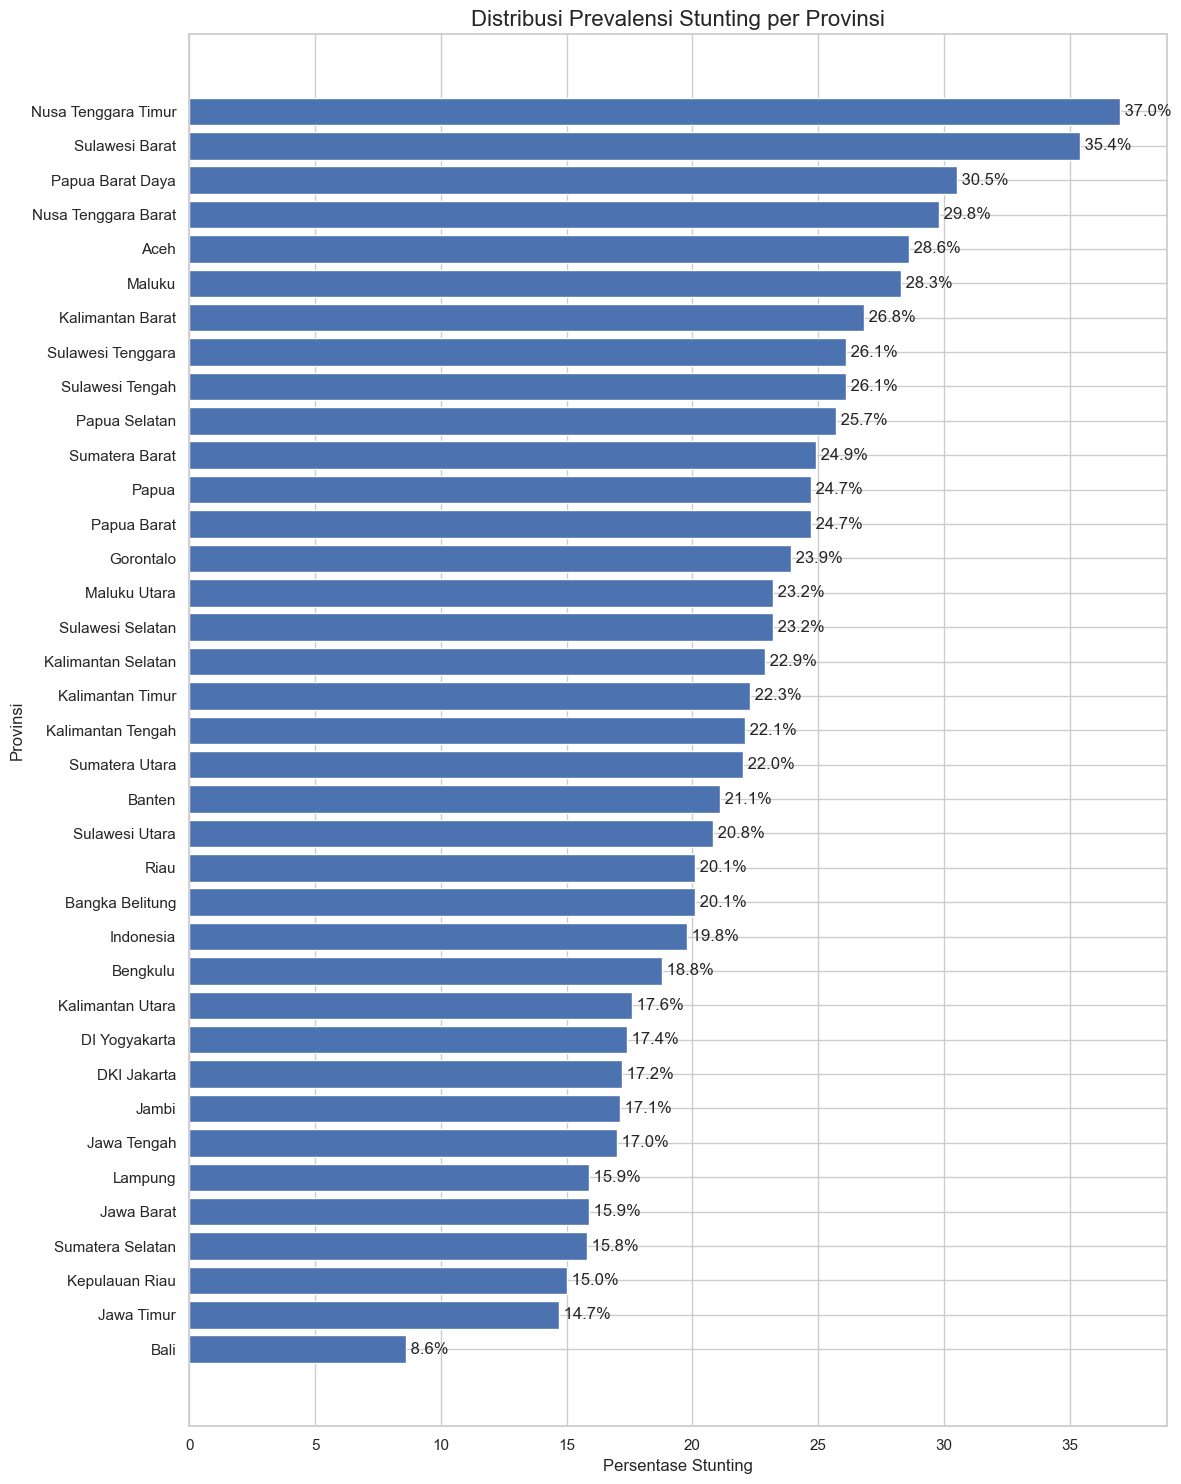
\includegraphics[width=0.95\textwidth]{figure/distribusi_stunting.png} 
    \caption{Distribusi Prevalensi \textit{Stunting} per Provinsi}
    \label{fig:eda_barchart}
\end{figure}

Visualisasi diagram batang pada Gambar \ref{fig:eda_barchart} merepresentasikan tingkat prevalensi \textit{stunting} di seluruh provinsi secara terurut. Berdasarkan grafik tersebut, Provinsi Nusa Tenggara Timur mencatatkan rekor angka tertinggi dengan persentase mencapai 37,0\%. Sebaliknya, Provinsi Bali menempati posisi terendah dengan tingkat prevalensi yang dapat ditekan hingga 8,6\%. Sementara itu, nilai rata-rata prevalensi secara agregat nasional berada pada angka 19,8\%. Pemetaan grafis ini memperlihatkan adanya ketimpangan status kesehatan balita yang cukup signifikan antarwilayah observasi di Indonesia.

\begin{figure}[H]
    \centering
    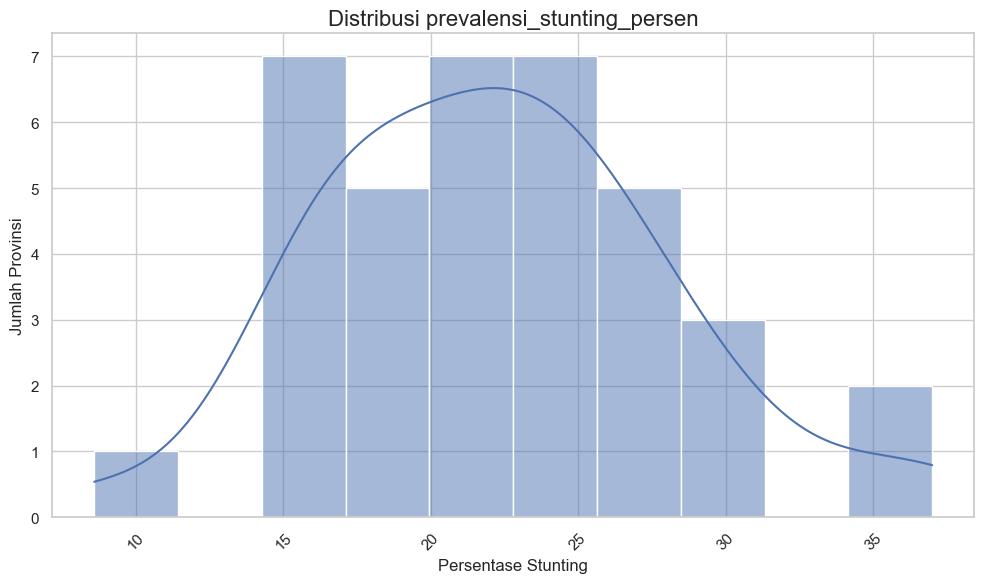
\includegraphics[width=0.85\textwidth]{figure/distribusi_persen.png}
    \caption{Histogram Distribusi Data Target}
    \label{fig:eda_histogram}
\end{figure}

Analisis sebaran frekuensi data target selanjutnya dijabarkan melalui bentuk histogram yang ditunjukkan pada Gambar \ref{fig:eda_histogram}. Kurva kepadatan pada grafik ini memperlihatkan pemusatan data (\textit{central tendency}) yang mendekati distribusi normal. Mayoritas provinsi di Indonesia memiliki tingkat prevalensi yang terkonsentrasi secara padat pada kelas interval 15\% hingga 25\%. Hanya terdapat sebagian kecil provinsi yang berada pada titik rentang ekstrem bawah maupun ekstrem atas. Pola distribusi ini mengonfirmasi bahwa masalah \textit{stunting} pada sebagian besar wilayah observasi cenderung seragam di sekitar nilai rata-rata.

Histogram pada gambar menunjukkan bahwa sebagian besar provinsi memiliki persentase yang berada pada rentang nilai tengah. Hal tersebut terlihat dari balok histogram dengan frekuensi paling tinggi yang terkonsentrasi di bagian tengah distribusi. Kurva distribusi yang berada di atas histogram juga memperlihatkan bahwa jumlah data semakin berkurang pada bagian kiri maupun kanan grafik. Selain itu, terdapat satu balok kecil pada sisi kanan histogram yang posisinya cukup terpisah dari kelompok data utama. Kondisi ini mengindikasikan adanya data dengan nilai yang jauh lebih tinggi dibandingkan data lainnya atau disebut sebagai \textit{outlier}. Secara umum, distribusi data yang terpusat pada nilai tengah seperti ini cukup baik karena dapat membantu algoritma \textit{machine learning} dalam mempelajari pola utama dari data latih secara lebih optimal.

\begin{figure}[H]
    \centering
    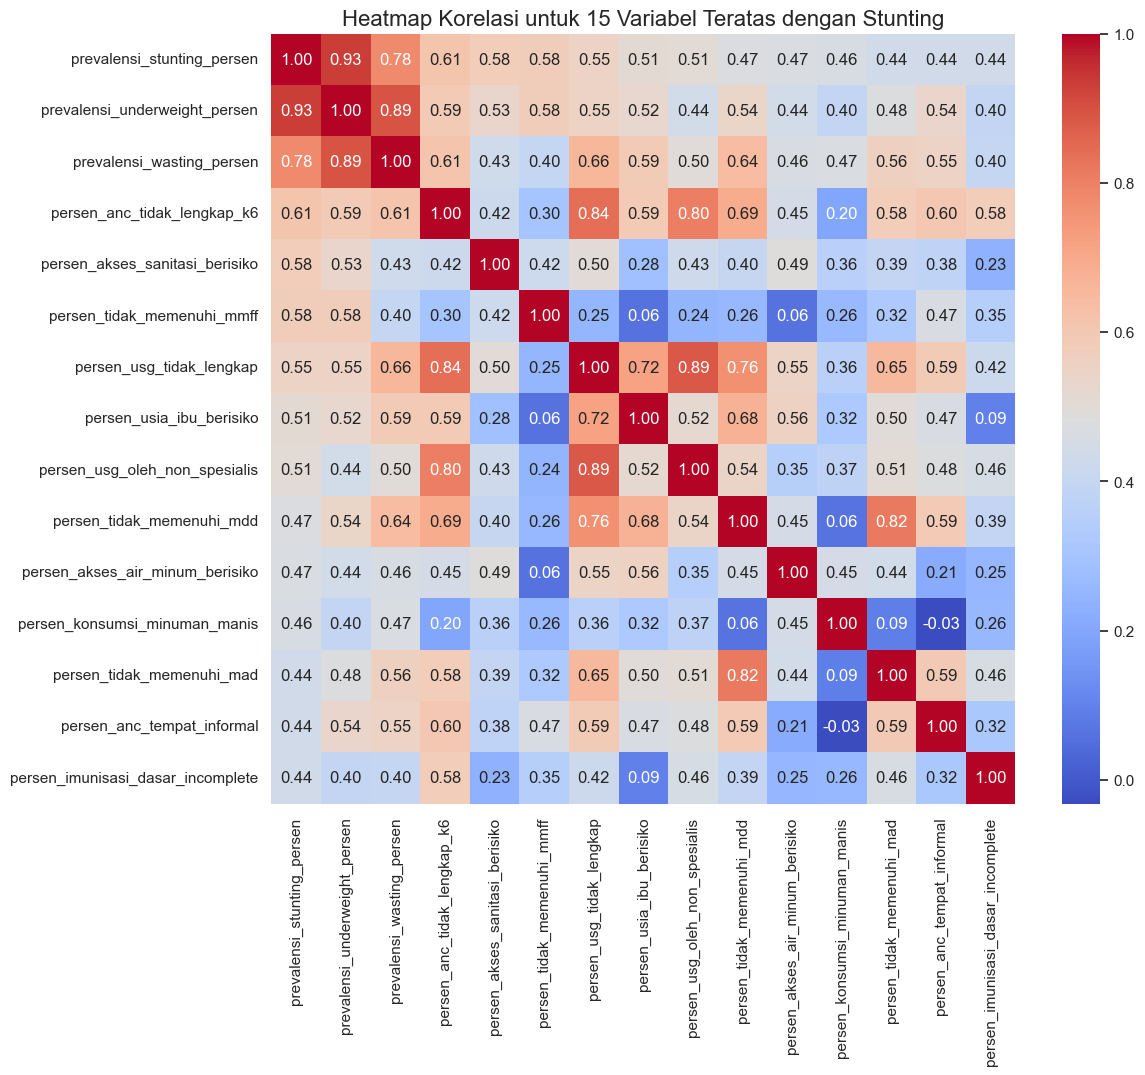
\includegraphics[width=0.95\textwidth]{figure/heatmap_korelasi.png}
    \caption{\textit{Heatmap} Korelasi 15 Variabel Teratas}
    \label{fig:eda_heatmap}
\end{figure}

Identifikasi hubungan linear antarvariabel diekstraksi menggunakan matriks korelasi \textit{Pearson} berbentuk \textit{heatmap} seperti yang tertera pada Gambar \ref{fig:eda_heatmap}. Baris pertama pada matriks tersebut secara spesifik memetakan nilai korelasi 15 kandidat fitur teratas terhadap variabel target prevalensi \textit{stunting}. Hasil perhitungan matematis menunjukkan hubungan positif yang sangat kuat dengan indikator malnutrisi lain, yakni \textit{underweight} (0,93) dan \textit{wasting} (0,78). Pada kategori fasilitas kesehatan dan lingkungan, fitur ketidaklengkapan pemeriksaan ANC K6 (0,61) serta risiko akses sanitasi (0,58) memegang peranan korelatif tertinggi. Temuan pola hubungan kuantitatif ini memberikan landasan objektif yang kuat untuk tahapan seleksi fitur sebelum masuk ke proses pemodelan.

\subsubsection{Penanganan \textit{Missing Value}}
Tahap penanganan \textit{missing value} dilakukan untuk memastikan integritas data sebelum memasuki fase pemodelan. Berdasarkan hasil temuan pada data mentah SSGI 2024, ditemukan kekosongan data yang masif pada Provinsi Papua Tengah dan Papua Pegunungan sebagai wilayah pemekaran baru. Karena ketiadaan data tersebut bersifat struktural pada level observasi, metode \textit{listwise deletion} diterapkan dengan menghapus kedua provinsi tersebut dari \textit{dataset}. Selain itu, baris agregat "Indonesia" juga dieliminasi karena bukan merupakan entitas provinsi independen. Langkah ini memastikan bahwa \textit{dataset} yang tersisa merupakan data lengkap tanpa memerlukan imputasi buatan. Implementasi kode dan ringkasan perubahan jumlah observasi ditunjukkan pada Kode 4.2 dan Tabel \ref{table:4.before_after_baris}.

\begin{lstlisting}[language=Python, caption={Penghapusan Observasi dan Validasi Missing Value}, label={code:missing_value}, frame=single, basicstyle=\ttfamily\scriptsize, breaklines=true]
# 1. Menghapus baris provinsi dengan data kosong dan agregat nasional
provinces_to_drop = ['Papua Tengah', 'Papua Pegunungan', 'Indonesia']

plot_data_clean = plot_data_clean[~plot_data_clean['Provinsi'] \
                                  .isin(provinces_to_drop)]

# 2. Validasi ketiadaan missing value
missing_values = plot_data_clean.isnull().sum()
missing_values = missing_values[missing_values > 0]

if len(missing_values) == 0:
    print("No missing values found in the dataset")
\end{lstlisting}

\begin{longtable}{|c|p{0.55\textwidth}|c|}
    \caption{Perbandingan Jumlah Observasi Sebelum dan Sesudah Pembersihan}
    \label{table:4.before_after_baris}\\
    \hline
    \centering\textbf{No} & \centering\textbf{Kondisi \textit{Dataset}} & \textbf{Jumlah Baris} \tabularnewline 
    \hline
    \endfirsthead
    \hline
    \centering\textbf{No} & \centering\textbf{Kondisi \textit{Dataset}} & \textbf{Jumlah Baris} \tabularnewline 
    \hline
    \endhead
    \hline
    \endfoot
    \hline
    \endlastfoot
    1 & Sebelum Penanganan \textit{Missing Value} & \centering 39 \tabularnewline 
    \hline
    2 & Sesudah Penanganan \textit{Missing Value} & \centering 36 \tabularnewline
    \hline
\end{longtable}

\subsubsection{Eliminasi Variabel Non-Determinan}
Setelah pembersihan baris, dilakukan eliminasi fitur pada tingkat kolom untuk menghindari bias pemodelan. Fitur \texttt{prevalensi\_underweight\_persen} dan \texttt{prevalensi\_wasting\_persen} dihapus secara sengaja karena merupakan indikator malnutrisi yang sangat berkorelasi dengan target \textit{stunting}. Mempertahankan kedua variabel ini akan memicu \textit{data leakage}, di mana model seolah-olah memiliki performa tinggi namun secara logika tidak valid dalam memetakan faktor penyebab (determinan) luar. Proses eliminasi ini dijabarkan pada Kode 4.3 dan perubahan dimensi kolomnya diringkas pada Tabel \ref{table:4.before_after_kolom}.

\begin{lstlisting}[language=Python, caption={Eliminasi Fitur untuk Mencegah \textit{Data Leakage}}, label={code:eliminasi_kolom}, frame=single, basicstyle=\ttfamily\scriptsize, breaklines=true]
# Menghapus kolom underweight dan wasting
columns_to_drop = ['prevalensi_underweight_persen', 'prevalensi_wasting_persen']
plot_data_clean = plot_data_clean.drop(columns=columns_to_drop)

print(f"Jumlah kolom setelah penghapusan: {len(plot_data_clean.columns)}")
\end{lstlisting}

\begin{longtable}{|c|p{0.55\textwidth}|c|}
    \caption{Perbandingan Jumlah Atribut Sebelum dan Sesudah Eliminasi}
    \label{table:4.before_after_kolom}\\
    \hline
    \centering\textbf{No} & \centering\textbf{Kondisi \textit{Dataset}} & \textbf{Jumlah Kolom} \tabularnewline 
    \hline
    \endfirsthead
    \hline
    \centering\textbf{No} & \centering\textbf{Kondisi \textit{Dataset}} & \textbf{Jumlah Kolom} \tabularnewline 
    \hline
    \endhead
    \hline
    \endfoot
    \hline
    \endlastfoot
    1 & Sebelum Eliminasi Variabel & \centering 58 \tabularnewline 
    \hline
    2 & Sesudah Eliminasi Variabel & \centering 56 \tabularnewline
    \hline
\end{longtable}

\subsubsection{Penetapan Variabel Penelitian}
Tahap akhir pra-pemrosesan adalah penetapan matriks variabel penelitian yang siap masuk ke tahap pemodelan. \textit{Dataset} final terdiri dari 36 provinsi dengan 54 fitur determinan numerik murni sebagai variabel independen ($X$) dan satu kolom target persentase prevalensi \textit{stunting} ($y$). Kolom nama provinsi dipisahkan karena tidak berperan dalam perhitungan matematis algoritma \textit{Random Forest}. Rincian pemisahan matriks ditunjukkan pada Kode 4.4, sedangkan struktur data finalnya direpresentasikan pada Tabel \ref{table:4.dataset_final}.

\begin{lstlisting}[language=Python, caption={Pemisahan Variabel Independen (X) dan Dependen (y)}, label={code:penetapan_variabel}, frame=single, basicstyle=\ttfamily\scriptsize, breaklines=true]
# Menentukan target dan fitur prediktor
y = plot_data_clean['prevalensi_stunting_persen']
X = plot_data_clean.drop(['Provinsi', 'prevalensi_stunting_persen'], axis=1)

print("Dimensi X:", X.shape) # (36, 54)
print("Dimensi y:", y.shape) # (36,)
\end{lstlisting}

\begin{longtable}{|c|p{0.18\textwidth}|p{0.18\textwidth}|p{0.18\textwidth}|c|}
    \caption{Ilustrasi \textit{Dataset} Final Pemodelan \textit{Stunting}}
    \label{table:4.dataset_final}\\
    \hline
    \centering\textbf{Provinsi} \newline \textit{(Index)} & \centering\textbf{y:} \newline \textbf{prevalensi\_} \newline \textbf{stunting} & \centering\textbf{X1:} \newline \textbf{jarak\_} \newline \textbf{hamil\_} \newline \textbf{risiko} & \centering\textbf{X2:} \newline \textbf{usia\_} \newline \textbf{ibu\_} \newline \textbf{risiko} & \textbf{... (X54)} \tabularnewline 
    \hline
    \endfirsthead
    \hline
    \centering\textbf{Provinsi} \newline \textit{(Index)} & \centering\textbf{y:} \newline \textbf{prevalensi\_} \newline \textbf{stunting} & \centering\textbf{X1:} \newline \textbf{jarak\_} \newline \textbf{hamil\_} \newline \textbf{risiko} & \centering\textbf{X2:} \newline \textbf{usia\_} \newline \textbf{ibu\_} \newline \textbf{risiko} & \textbf{... (X54)} \tabularnewline 
    \hline
    \endhead
    \hline
    \endfoot
    \hline
    \endlastfoot
    Bali & \centering 8,6 & \centering 9,5 & \centering 12,5 & ... \tabularnewline 
    \hline
    Jawa Timur & \centering 14,7 & \centering 10,4 & \centering 13,1 & ... \tabularnewline
    \hline
    Kep. Riau & \centering 15,0 & \centering 10,6 & \centering 10,3 & ... \tabularnewline
    \hline
    ... & \centering ... & \centering ... & \centering ... & ... \tabularnewline
    \hline
\end{longtable}

\subsection{Pemodelan \textit{Random Forest}}
Setelah melalui serangkaian tahapan pra-pemrosesan data, langkah selanjutnya adalah pengembangan algoritma untuk memprediksi angka prevalensi \textit{stunting}. Mengacu pada alur penelitian, rangkaian proses pengembangan model dibagi menjadi tiga tahapan utama, mulai dari pencarian parameter optimal (\textit{hyperparameter tuning}), pelatihan model secara utuh (\textit{fitting}), hingga diakhiri dengan evaluasi performa model. Adapun proses-proses tersebut dijabarkan sebagai berikut.

\subsubsection{\textit{Hyperparameter Tuning} Berbasis \textit{Cross Validation}}
Tahapan \textit{hyperparameter tuning} dilaksanakan dengan tujuan mengidentifikasi konfigurasi optimal pada model \textit{Random Forest Regressor} agar mampu menghasilkan performa prediksi yang stabil dan akurat. Mengingat dimensi \textit{dataset} penelitian yang tergolong kecil (36 observasi), pembagian data latih (\textit{training}) dan data uji (\textit{testing}) konvensional berisiko menghasilkan variansi bias yang tinggi. Oleh karena itu, pendekatan \textit{Leave-One-Out Cross-Validation} (LOOCV) diterapkan. Pada skema ini, model dilatih sebanyak 36 kali, di mana pada setiap iterasinya, 35 data digunakan untuk pelatihan dan 1 data ditinggalkan untuk pengujian. Bersamaan dengan proses ini, dilakukan pencarian parameter terbaik menggunakan \textit{Grid Search} terhadap 108 kombinasi parameter. Evaluasi kinerja difokuskan untuk menekan nilai \textit{Mean Absolute Error} (MAE).

Secara konseptual, tahapan pencarian parameter melalui skema LOOCV ini merupakan fase di mana proses pelatihan (\textit{training}), validasi (\textit{validation}), dan pengujian (\textit{testing}) dieksekusi secara serentak di dalam satu siklus iterasi terintegrasi. Melalui pendekatan ini, evaluasi performa model dapat dilakukan secara menyeluruh terhadap data yang disembunyikan (\textit{unseen data}) pada setiap iterasinya tanpa memerlukan pemisahan proporsi data di awal, sehingga representasi informasi penting dari keseluruhan populasi sampel tetap terjaga. Rincian proses komputasi iteratif beserta ekstraksi matriks evaluasi pada tahapan ini dijabarkan pada Kode 4.5.

\begin{lstlisting}[language=Python, caption={Pelaksanaan LOOCV, Grid Search, dan Ekstraksi Evaluasi}, label={code:tuning}, frame=single, basicstyle=\ttfamily\scriptsize, breaklines=true]
from sklearn.model_selection import GridSearchCV, LeaveOneOut
from sklearn.ensemble import RandomForestRegressor

# Definisi kandidat parameter
param_grid = {
    'n_estimators': [50, 100, 150],
    'max_depth': [3, 5, 7, None],
    'min_samples_leaf': [1, 2, 3],
    'max_features': ['sqrt', 'log2', None]
}

model = RandomForestRegressor(random_state=42)
loocv = LeaveOneOut()
scorers = {'mae': 'neg_mean_absolute_error', 
           'rmse': 'neg_root_mean_squared_error'}

# Eksekusi Grid Search dengan LOOCV
grid_search = GridSearchCV(
    estimator=model, param_grid=param_grid, cv=loocv, 
    scoring=scorers, refit='mae', return_train_score=True, n_jobs=-1, verbose=2)

grid_search.fit(X, y)

# Ekstraksi dan peninjauan skor terbaik berdasarkan MAE
best_index = grid_search.best_index_
best_mae = -grid_search.cv_results_['mean_test_mae'][best_index]
best_rmse = -grid_search.cv_results_['mean_test_rmse'][best_index]

print(f"Kombinasi Parameter Optimal: {grid_search.best_params_}")
print(f"Skor MAE Terbaik: {best_mae:.2f}")
print(f"Skor RMSE Terbaik: {best_rmse:.2f}")
\end{lstlisting}

Hasil komputasi dari pencarian parameter optimal secara komprehensif direpresentasikan pada Tabel \ref{table:4.best_param}. Berdasarkan matriks evaluasi, konfigurasi terbaik untuk algoritma \textit{Random Forest Regressor} diperoleh pada kombinasi penggunaan 100 estimasi pohon (\texttt{n\_estimators}), kedalaman maksimal 5 tingkat (\texttt{max\_depth}), batas minimal 1 observasi pada simpul daun (\texttt{min\_samples\_leaf}), dan fungsi logaritma basis 2 untuk penyeleksian fitur maksimal (\texttt{max\_features}). Penerapan pengaturan parameter tersebut secara komputasional menghasilkan tingkat penyimpangan prediksi terendah dengan skor \textit{Mean Absolute Error} (MAE) dan \textit{Root Mean Squared Error} (RMSE) yang masing-masing bernilai 3,44. Konsistensi perolehan angka minimal pada kedua metrik evaluasi tersebut mengonfirmasi tingkat stabilitas model dalam mengenali pola data. 

\begin{longtable}{|c|p{0.4\textwidth}|c|}
    \caption{Hasil \textit{Hyperparameter Tuning} Model \textit{Random Forest}}
    \label{table:4.best_param}\\
    \hline
    \centering\textbf{No} & \centering\textbf{Nama Parameter} & \textbf{Nilai Optimal} \tabularnewline 
    \hline
    \endfirsthead
    \hline
    \centering\textbf{No} & \centering\textbf{Nama Parameter} & \textbf{Nilai Optimal} \tabularnewline 
    \hline
    \endhead
    \hline
    \endfoot
    \hline
    \endlastfoot
    1 & \texttt{n\_estimators} & \centering 100 \tabularnewline 
    \hline
    2 & \texttt{max\_depth} & \centering 5 \tabularnewline
    \hline
    3 & \texttt{min\_samples\_leaf} & \centering 1 \tabularnewline
    \hline
    4 & \texttt{max\_features} & \centering \texttt{log2} \tabularnewline
    \hline
\end{longtable}

Selanjutnya, untuk memvalidasi stabilitas performa model secara visual, dinamika perbandingan tingkat kesalahan selama proses pencarian parameter ditunjukkan melalui kurva pembelajaran (\textit{learning curve}) pada Gambar \ref{fig:learning_curve}. Berdasarkan grafik tersebut, evaluasi LOOCV mencapai titik kesalahan terendah pada iterasi kombinasi parameter ke-38, yang secara visual ditandai dengan titik merah. Konsistensi pergerakan jarak antara kurva pelatihan dan validasi tanpa adanya lonjakan deviasi yang ekstrem mengonfirmasi bahwa konfigurasi optimal yang dipilih mampu menjaga model dari \textit{overfitting} secara berlebihan.

\begin{figure}[H]
    \centering
    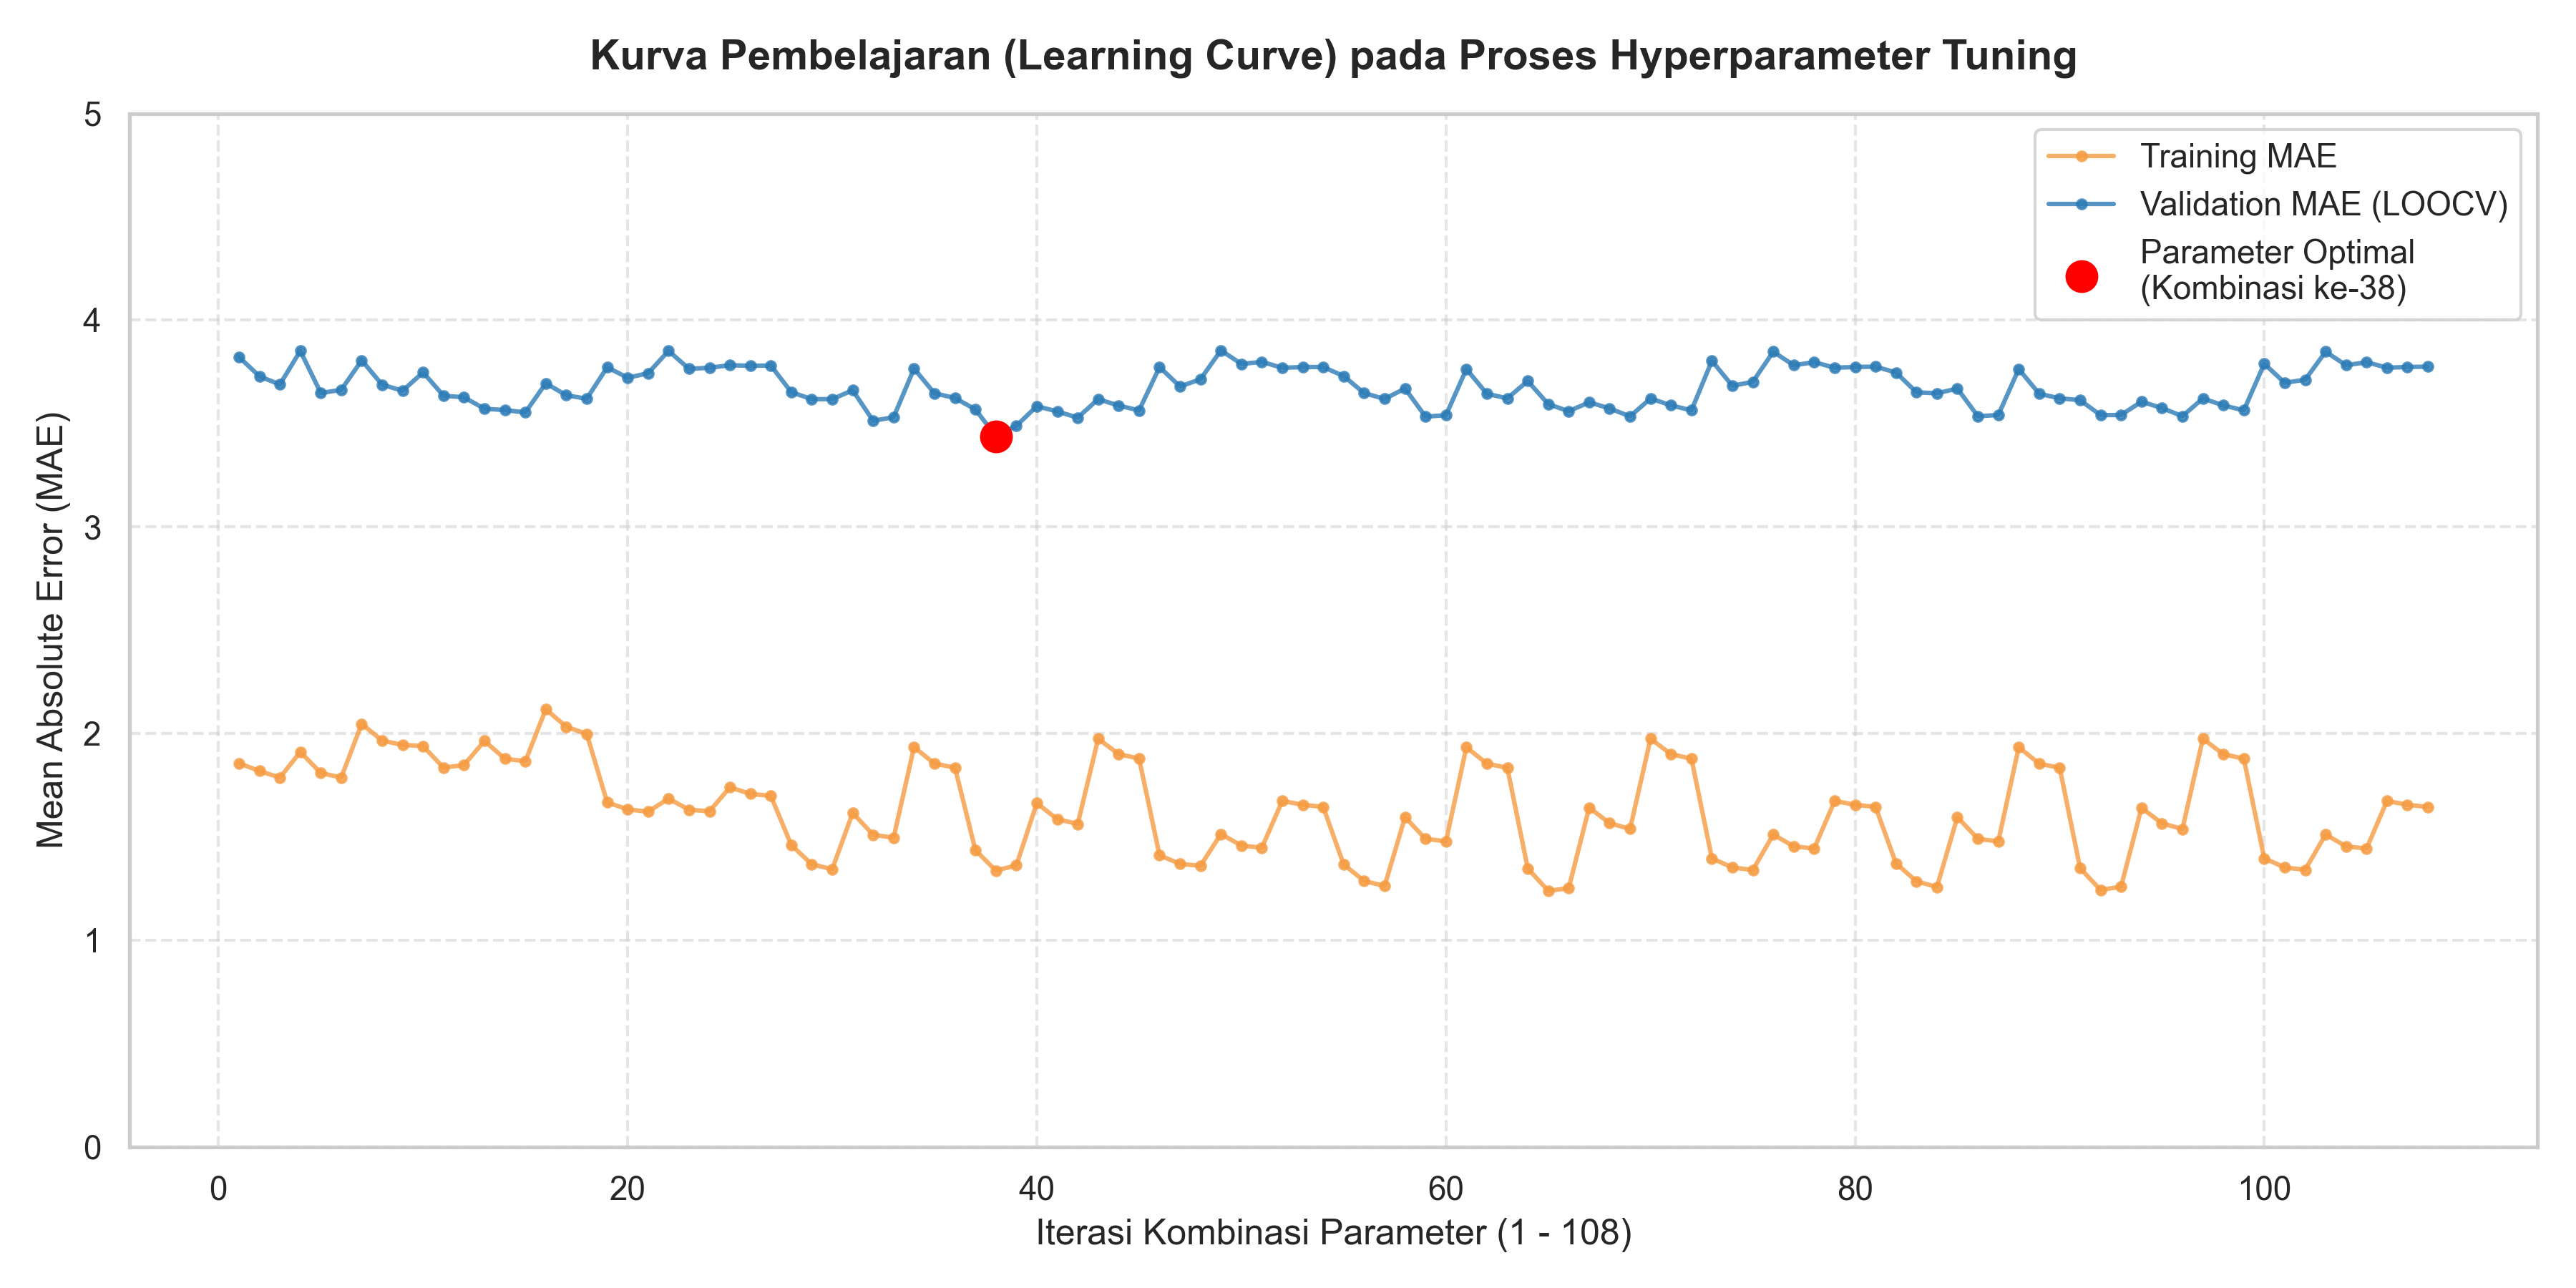
\includegraphics[width=0.85\textwidth]{figure/learning_curve_tuning.png} 
    \caption{Kurva Pelatihan dan Validasi pada Proses \textit{Hyperparameter Tuning}}
    \label{fig:learning_curve}
\end{figure}

\subsubsection{Pelatihan Model Final}
Setelah konfigurasi parameter terbaik berhasil diidentifikasi pada tahapan sebelumnya, proses dilanjutkan dengan pembentukan model final. Parameter optimal yang diperoleh dari proses \textit{tuning} tersebut kemudian dikonfigurasikan ke dalam algoritma \textit{Random Forest Regressor} yang baru. Model final ini dilatih kembali (\textit{retrain}) menggunakan keseluruhan 36 baris \textit{dataset} populasi untuk mendapatkan pola pemetaan variabel fitur secara maksimal tanpa adanya reduksi sampel. Setelah model berhasil dilatih secara utuh, dilakukan prediksi terhadap nilai prevalensi \textit{stunting} guna membandingkan kedekatan antara nilai target aktual dengan nilai tebakan dari sistem. Rincian implementasi deklarasi model dan eksekusi prediksi dapat dilihat pada Kode 4.6. Selanjutnya, sintaksis komputasi untuk memvisualisasikan sebaran kedekatan tersebut ditunjukkan pada Kode 4.7, dengan hasil komparasi aktual-prediksi direpresentasikan pada Tabel \ref{table:4.komparasi_prediksi} dan Gambar \ref{fig:visualisasi_prediksi}.

\begin{lstlisting}[language=Python, caption={Pelatihan Model dan Eksekusi Prediksi}, label={code:pelatihan_final}, frame=single, basicstyle=\ttfamily\scriptsize, breaklines=true]
import pandas as pd
import matplotlib.pyplot as plt

# Deklarasi model final dengan parameter terbaik
best_params = grid_search.best_params_
model_final = RandomForestRegressor(**best_params, random_state=42)

# Melatih model dengan seluruh observasi
model_final.fit(X, y)

# Melakukan prediksi pada data
y_pred = model_final.predict(X)

# Menyusun DataFrame komparasi
comparison_df = pd.DataFrame({
    'Provinsi': plot_data_clean['Provinsi'],
    'Actual': y, 'Predicted': y_pred,
    'Difference': y - y_pred
}).sort_values('Actual')

pd.set_option('display.float_format', lambda x: '%.2f' % x)
\end{lstlisting}

\begin{longtable}{|c|p{0.25\textwidth}|p{0.14\textwidth}|p{0.14\textwidth}|p{0.14\textwidth}|}
    \caption{Cuplikan Perbandingan Nilai Aktual dan Prediksi}
    \label{table:4.komparasi_prediksi}\\
    \hline
    \centering\textbf{No} & \centering\textbf{Provinsi} & \centering\textbf{Aktual} & \centering\textbf{Prediksi} & \centering\textbf{Selisih} \tabularnewline 
    \hline
    \endfirsthead
    \hline
    \centering\textbf{No} & \centering\textbf{Provinsi} & \centering\textbf{Aktual} & \centering\textbf{Prediksi} & \centering\textbf{Selisih} \tabularnewline 
    \hline
    \endhead
    \hline
    \endfoot
    \hline
    \endlastfoot
    1 & Bali & \centering 8,60 & \centering 12,56 & \centering -3,96 \tabularnewline 
    \hline
    2 & Jawa Timur & \centering 14,70 & \centering 16,77 & \centering -2,07 \tabularnewline
    \hline
    3 & Kep. Riau & \centering 15,00 & \centering 16,96 & \centering -1,96 \tabularnewline
    \hline
    \multicolumn{5}{|c|}{\textit{... }} \tabularnewline
    \hline
    35 & Sulawesi Barat & \centering 35,40 & \centering 31,28 & \centering 4,12 \tabularnewline
    \hline
    36 & NTT & \centering 37,00 & \centering 33,82 & \centering 3,18 \tabularnewline
    \hline
\end{longtable}

Rincian komparasi numerik pada Tabel \ref{table:4.komparasi_prediksi} tersebut memberikan gambaran awal mengenai tingkat simpangan yang dihasilkan oleh model final. Agar mempermudah observasi terhadap pola sebaran selisih data secara komprehensif, hasil perbandingan antara nilai prevalensi \textit{stunting} aktual dan tebakan prediksi divisualisasikan secara utuh pada Gambar \ref{fig:visualisasi_prediksi}. Representasi grafis ini memetakan kedekatan kedua nilai tersebut pada masing-masing dari 36 provinsi agar performa akurasi sistem dapat diinterpretasikan dengan lebih intuitif.

\begin{figure}[H]
    \centering
    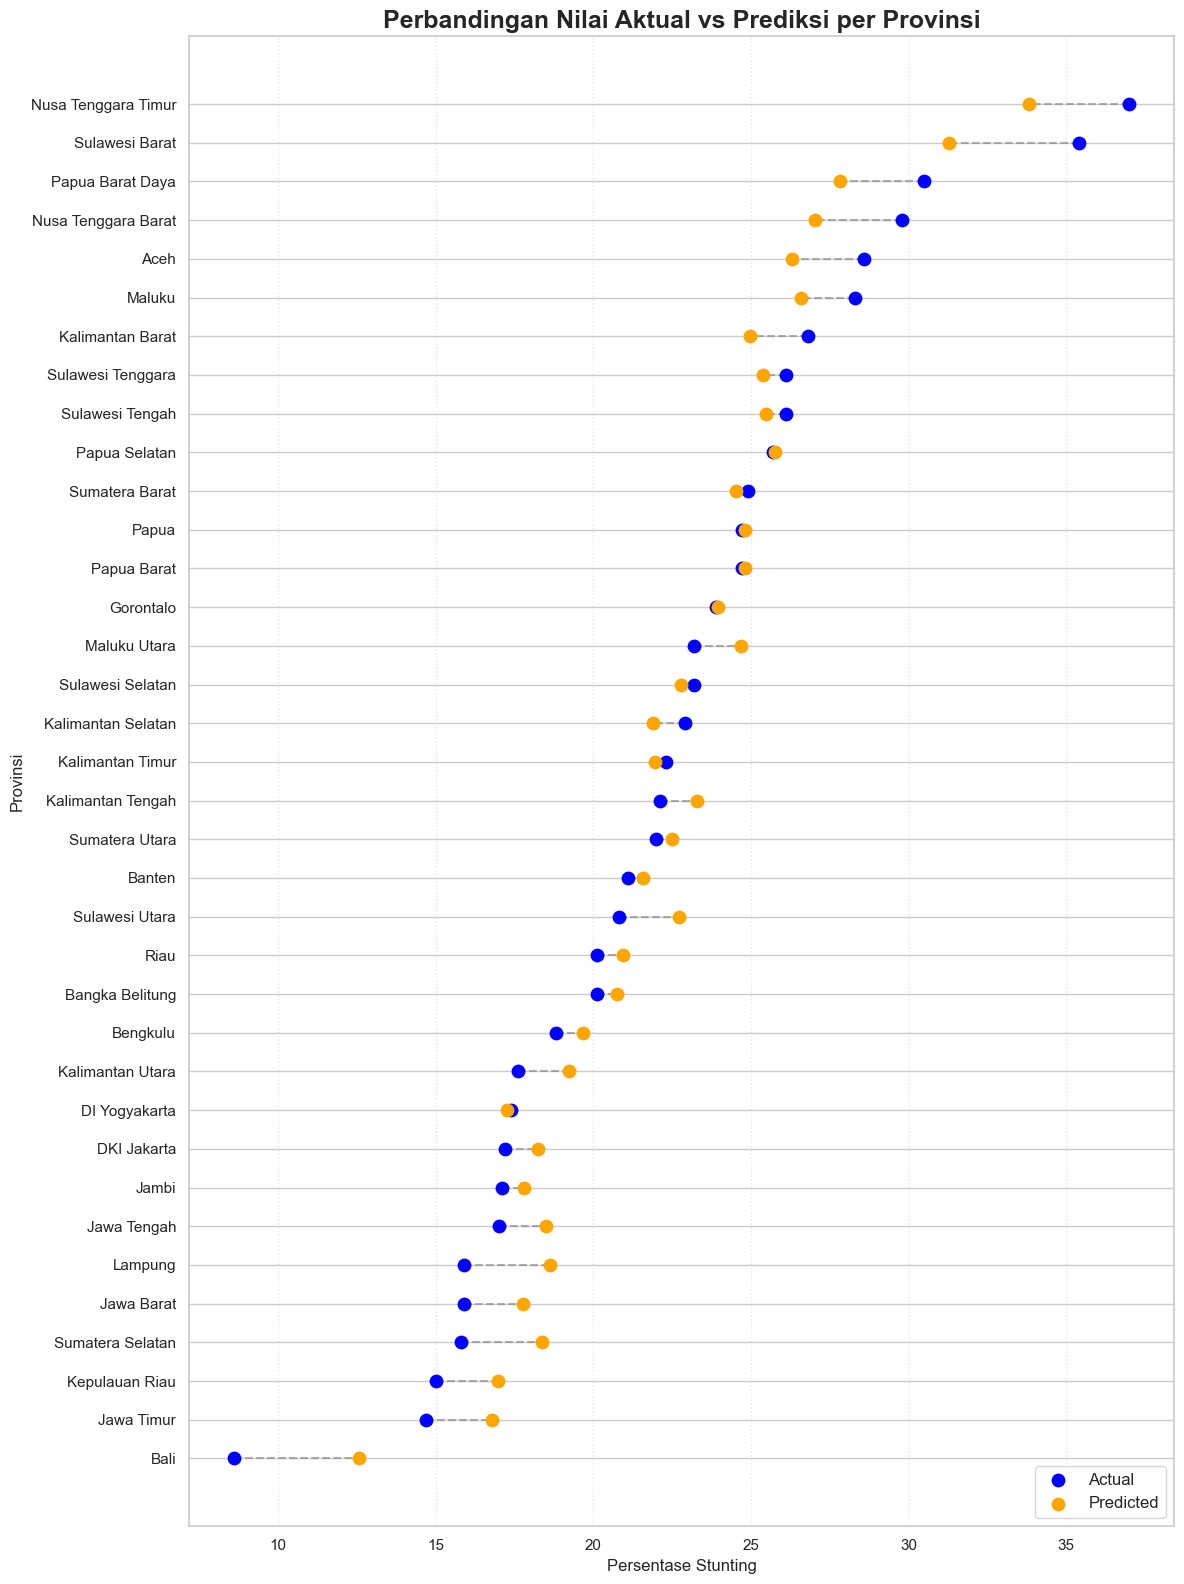
\includegraphics[width=0.8\textwidth]{figure/pred_act.png} 
    \caption{Sebaran Nilai Aktual dan Prediksi \textit{Stunting} per Provinsi}
    \label{fig:visualisasi_prediksi}
\end{figure}

\section{Evaluasi Performa Model}
Tahapan evaluasi performa algoritma \textit{Random Forest} pada penelitian ini dibagi menjadi dua skema pengukuran utama. Skema pertama berfokus pada pengujian generalisasi saat fase \textit{tuning} parameter menggunakan LOOCV sebagai metrik performa utama. Skema kedua mengukur tingkat pencocokan model referensi pada populasi data utuh sebelum ekstraksi nilai SHAP dilakukan.

\subsection{Hasil Evaluasi Generalisasi (LOOCV)}
Pengukuran performa generalisasi dieksekusi menggunakan skema LOOCV sebanyak 36 iterasi. Metode ini menguji algoritma secara berulang dengan menahan satu provinsi sebagai data uji secara bergantian. Rincian ekstraksi metrik generalisasi dari log komputasi ini dieksekusi melalui sintaksis pada Kode 4.7.

\begin{lstlisting}[language=Python, caption={Ekstraksi Metrik Evaluasi Generalisasi LOOCV}, label={code:loocv_eval}, frame=single, basicstyle=\ttfamily\scriptsize, breaklines=true]
# Get scores for both metrics
mae_scores = -grid_search.cv_results_['mean_test_mae']
rmse_scores = -grid_search.cv_results_['mean_test_rmse']

# Get the index of the best model
best_index = grid_search.best_index_

print("\nBest model scores:")
print(f"MAE: {mae_scores[best_index]:.4f}")
print(f"RMSE: {rmse_scores[best_index]:.4f}")
\end{lstlisting}

Berdasarkan rekaman log komputasi pada Kode 4.7, konfigurasi parameter terbaik menghasilkan rata-rata MAE uji sebesar 3,44. Nilai RMSE uji juga tercatat pada angka yang sama, yaitu sebesar 3,44. Angka ini secara mutlak menjadi acuan utama dalam menilai kemampuan generalisasi algoritma terhadap observasi baru. Rincian metrik performa generalisasi tersebut disajikan secara ringkas pada Tabel \ref{table:4.hasil_loocv}.

\begin{longtable}{|c|p{0.55\textwidth}|c|}
    \caption{Hasil Evaluasi Generalisasi (LOOCV)}
    \label{table:4.hasil_loocv}\\
    \hline
    \textbf{No} & \multicolumn{1}{c|}{\textbf{Metrik Evaluasi}} & \textbf{Skor} \tabularnewline 
    \hline
    \endfirsthead
    \hline
    \textbf{No} & \multicolumn{1}{c|}{\textbf{Metrik Evaluasi}} & \textbf{Skor} \tabularnewline 
    \hline
    \endhead
    \hline
    \endfoot
    \hline
    \endlastfoot
    1 & MAE & 3,44 \tabularnewline 
    \hline
    2 & RMSE & 3,44 \tabularnewline
    \hline
\end{longtable}

\subsection{Hasil Evaluasi Model Referensi (\textit{Full-Training})}
Tahapan evaluasi selanjutnya dilakukan semata-mata untuk meninjau seberapa baik algoritma berhasil memetakan variabel fitur terhadap target aktualnya. Sesuai dengan skema fase kedua, model final ini telah dilatih menggunakan 100\% observasi tanpa adanya data yang disembunyikan. Pendekatan evaluasi dilakukan melalui perhitungan matematis antara nilai tebakan model (\texttt{y\_pred}) dan data realita (\texttt{y}). Rincian sintaksis komputasi untuk kalkulasi metrik evaluasi dieksekusi pada Kode 4.8.

\begin{lstlisting}[language=Python, caption={Perhitungan Metrik Evaluasi Regresi}, label={code:evaluasi}, frame=single, basicstyle=\ttfamily\scriptsize, breaklines=true]
from sklearn.metrics import mean_absolute_error, mean_squared_error, r2_score
import numpy as np

# Mengkalkulasi nilai metrik evaluasi
mae = mean_absolute_error(y, y_pred)
mse = mean_squared_error(y, y_pred)
rmse = np.sqrt(mse)
r2 = r2_score(y, y_pred)
mape = np.mean(np.abs((y - y_pred) / y)) * 100

print(f"MAE: {mae:.2f} | RMSE: {rmse:.2f}")
print(f"R-squared: {r2:.4f} | MAPE: {mape:.2f}%")
\end{lstlisting}

Berdasarkan hasil komputasi pada Tabel \ref{table:4.hasil_evaluasi}, model \textit{Random Forest} mampu merekam pola \textit{dataset} latih dengan nilai determinasi ($R^2$) sebesar 0,9090. Skor ini mengindikasikan bahwa algoritma dapat menjelaskan 90,9\% variabilitas penyebab \textit{stunting} pada data pelatihan secara proporsional. Di sisi lain, persentase deviasi prediksi yang ditunjukkan oleh nilai MAPE mencatatkan angka 7,22\%. Rincian komprehensif dari hasil evaluasi pencocokan model referensi ini disajikan secara lengkap pada Tabel \ref{table:4.hasil_evaluasi}. Penting untuk dicatat bahwa seluruh angka tersebut merepresentasikan performa \textit{in-sample} yang sama sekali tidak bisa dijadikan acuan generalisasi.

\begin{longtable}{|c|p{0.55\textwidth}|c|}
    \caption{Hasil Evaluasi Pencocokan Model Referensi (Data Latih Utuh)}
    \label{table:4.hasil_evaluasi}\\
    \hline
    \textbf{No} & \multicolumn{1}{c|}{\textbf{Metrik Evaluasi}} & \textbf{Skor} \tabularnewline 
    \hline
    \endfirsthead
    \hline
    \textbf{No} & \multicolumn{1}{c|}{\textbf{Metrik Evaluasi}} & \textbf{Skor} \tabularnewline 
    \hline
    \endhead
    \hline
    \endfoot
    \hline
    \endlastfoot
    1 & MAE & 1,40 \tabularnewline 
    \hline
    2 & RMSE & 1,77 \tabularnewline
    \hline
    3 & $R^2$ & 0,9090 \tabularnewline
    \hline
    4 & MAPE & 7,22\% \tabularnewline
    \hline
\end{longtable}

\section{Analisis Hasil Pemodelan \textit{Random Forest}}
Setelah semua tahapan pembuatan model dan pengujian selesai dilakukan, bagian ini akan membahas hasil yang diperoleh. Analisis ini bertujuan untuk meninjau kecocokan pengaturan parameter, pola prediksi model, dan nilai evaluasinya. Pembahasan ini penting sebagai pengantar yang logis sebelum masuk ke tahap interpretasi fitur menggunakan SHAP. Rincian analisis tersebut dijelaskan pada poin-poin berikut.

\subsection{Analisis Konfigurasi Parameter}
Tahap konfigurasi parameter membahas kecocokan hasil \textit{tuning} optimal yang sebelumnya telah dirangkum pada Tabel \ref{table:4.best_param}. Pemilihan nilai \textit{max\_depth} sebesar 5 menunjukkan bahwa pembatasan kedalaman pohon efektif untuk \textit{dataset} dengan jumlah observasi yang sedikit. Langkah ini dilakukan untuk mencegah algoritma menghafal data latih secara berlebihan. Selain itu, penggunaan parameter \textit{max\_features} berupa \textit{log2} memastikan setiap variabel memiliki kesempatan yang sama untuk dievaluasi pada tiap cabang pohon. Pengaturan ini membantu model agar belajar lebih baik dan terhindar dari masalah \textit{overfitting}.

\subsection{Analisis Pola Prediksi \textit{Stunting} per Provinsi}
Pola tebakan model dapat diamati melalui komparasi pada Tabel \ref{table:4.komparasi_prediksi} dan visualisasi \textit{scatter plot} pada Gambar \ref{fig:visualisasi_prediksi}. Secara umum, garis prediksi menunjukkan tren yang sejalan dengan nilai aslinya di sebagian besar wilayah. Namun, masih terdapat sedikit perbedaan estimasi pada provinsi dengan tingkat prevalensi terendah seperti Bali, dan tertinggi seperti Nusa Tenggara Timur. Hal ini terjadi karena algoritma \textit{Random Forest} bekerja dengan cara mengambil nilai rata-rata dari banyak pohon keputusan. Cara kerja ini membuat prediksi model menjadi lebih stabil dan tidak mudah terpengaruh oleh data ekstrem (\textit{outlier}).

\subsection{Analisis Metrik Evaluasi}
Tingkat keberhasilan algoritma dalam mempelajari pola \textit{dataset} dianalisis dari segi ketahanan generalisasi dan kualitas pencocokan. Pembahasan ini mencakup tinjauan secara terpisah untuk kedua skema pengujian yang telah dilakukan. Langkah ini diambil secara khusus untuk menghindari kesalahan pemahaman terhadap performa asli algoritma \textit{machine learning} yang dibangun.

\subsubsection{Analisis Evaluasi Generalisasi (LOOCV)}
Pada tahap generalisasi melalui LOOCV, diperoleh nilai MAE uji sebesar 3,44 yang ditetapkan sebagai metrik utama performa model. Kesamaan angka antara MAE dan RMSE pada pengujian ini terjadi secara matematis akibat sifat dari skema sampel uji tunggal. Pada kondisi lipatan dengan jumlah data uji hanya satu ($n=1$), hasil perhitungan kuadrat \textit{error} secara mutlak akan selalu setara dengan nilai absolutnya. Angka ini secara objektif menjadi tolok ukur penyimpangan tebakan sistem jika dihadapkan pada observasi provinsi baru.

\subsubsection{Analisis Pencocokan Model (\textit{Full-Training})}
Pada tahap evaluasi model referensi utuh, skor $R^2$ tercatat sebesar 0,9090 untuk keseluruhan data. Hal ini mengonfirmasi bahwa kumpulan variabel prediktor mampu merekam variabilitas determinan \textit{stunting} secara proporsional pada data latih. Harus ditekankan secara eksplisit bahwa nilai $R^2$ tersebut adalah \textit{training in-sample} yang tidak bisa dijadikan acuan generalisasi. Model final ini difokuskan hanya sebagai referensi interpretasi dan bukan dideklarasikan untuk ekstrapolasi observasi baru. Di sisi lain, algoritma berbasis \textit{ensemble} ini memiliki sifat \textit{black-box} sehingga tahapan selanjutnya dikhususkan untuk mengekstraksi arah kontribusi fitur menggunakan SHAP.

\section{Interpretasi Model Menggunakan SHAP}
Mengacu pada batasan algoritma \textit{Random Forest} yang bersifat kotak hitam, tahapan ini difokuskan pada interpretasi hasil prediksi menggunakan SHAP. Pendekatan ini digunakan untuk mengetahui besaran pengaruh dari masing-masing variabel independen terhadap angka prevalensi \textit{stunting}. Analisis SHAP dalam penelitian ini dibagi menjadi dua ruang lingkup, yaitu analisis skala global dan analisis skala lokal. Pembagian ini bertujuan untuk melihat gambaran besar faktor penentu di tingkat nasional, sekaligus mengamati alasan spesifik di balik hasil prediksi pada masing-masing provinsi.

Proses interpretasi diawali dengan menginisialisasi objek pembaca model (\textit{explainer}) ke dalam sistem. Karena \textit{Random Forest} merupakan algoritma yang dibangun dari sekumpulan pohon keputusan, pustaka SHAP menyediakan fungsi khusus berupa \texttt{TreeExplainer} untuk membaca struktur model tersebut secara efisien. Setelah model berhasil dibaca, sistem akan menghitung matriks nilai SHAP untuk mengukur seberapa besar dorongan atau tarikan setiap variabel terhadap hasil tebakan akhir. Rincian deklarasi algoritma SHAP beserta pengecekan dimensi \textit{output}-nya ditunjukkan pada Kode 4.9.

\begin{lstlisting}[language=Python, caption={Inisialisasi TreeExplainer dan Ekstraksi Nilai SHAP}, label={code:shap_init}, frame=single, basicstyle=\ttfamily\scriptsize, breaklines=true]
import shap
import numpy as np

# Inisialisasi SHAP explainer untuk model berbasis pohon
explainer = shap.TreeExplainer(model_final)
shap_values = explainer.shap_values(X)

# Pengecekan dimensi matriks SHAP values
print("Dimensi SHAP values:", np.shape(shap_values))
# Output: (36, 54)
\end{lstlisting}

\subsection{Interpretasi Global (\textit{Global Explanation})}
Interpretasi skala global bertujuan untuk melihat pola pengambilan keputusan model terhadap seluruh data observasi tingkat nasional. Pendekatan ini berfokus pada evaluasi dampak masing-masing variabel secara umum sebelum meninjau kasus pada wilayah yang lebih spesifik. Proses interpretasi model pada tahapan ini dibagi ke dalam tiga bentuk visualisasi utama. Visualisasi tersebut mencakup identifikasi urutan variabel penentu, pengamatan arah pengaruh fitur, dan peninjauan batas angka kritis dari indikator utama. Rincian penjelasan untuk masing-masing tahapan analisis ini diuraikan pada sub-subbab berikut.

\subsubsection{Tingkat Kepentingan Fitur (\textit{Feature Importance Plot})}
Tahap awal interpretasi dilakukan dengan mengekstraksi tingkat kepentingan fitur melalui perhitungan rata-rata nilai absolut SHAP. Hasil komputasi pada Kode 4.10 divisualisasikan dalam bentuk diagram batang pada Gambar \ref{fig:shap_bar} yang secara spesifik dibatasi hanya untuk menampilkan 20 fitur dengan kontribusi tertinggi guna menjaga keterbacaan dokumen. Melalui pembatasan grafik ini, urutan indikator determinan yang menjadi penentu utama prevalensi \textit{stunting} dapat diidentifikasi secara eksplisit.

\begin{lstlisting}[language=Python, caption={Visualisasi Tingkat Kepentingan Fitur Global}, label={code:shap_bar}, frame=single, basicstyle=\ttfamily\scriptsize, breaklines=true]
import matplotlib.pyplot as plt

# Visualisasi Bar Plot untuk 20 fitur paling berpengaruh
shap.summary_plot(shap_values, X, plot_type="bar", 
                  max_display=20, show=False)

fig = plt.gcf()
fig.set_size_inches(10, 8)
plt.title("Rata-rata Dampak Absolut Fitur terhadap Stunting", fontsize=14)
plt.tight_layout()
plt.show()
\end{lstlisting}

\begin{figure}[H]
    \centering
    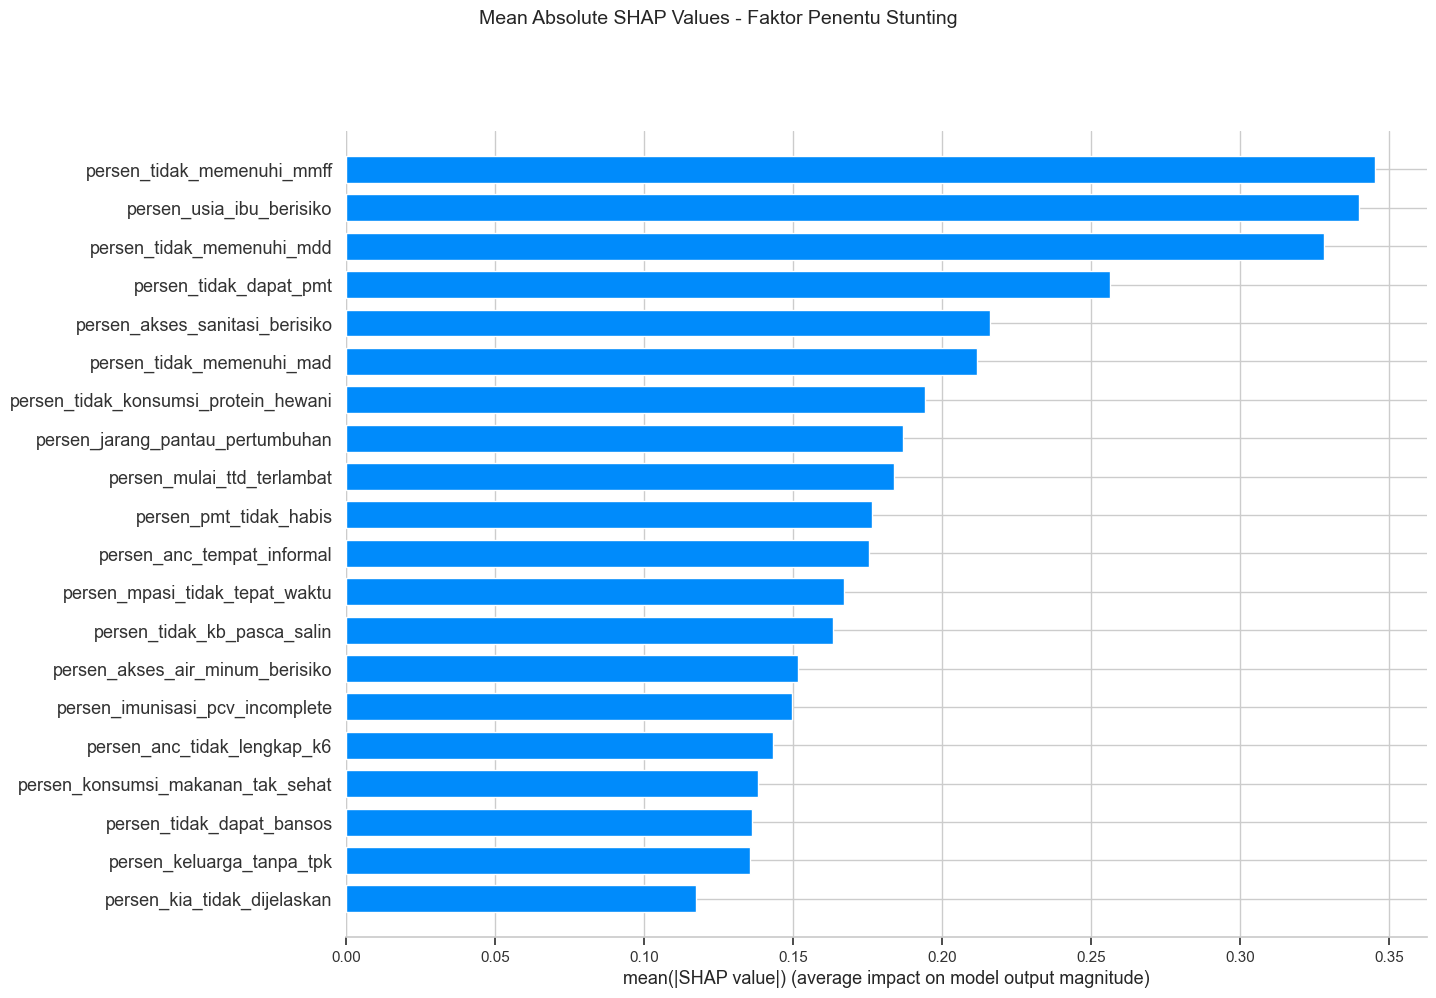
\includegraphics[width=0.85\textwidth]{figure/feature_importance.png} 
    \caption{Rata-Rata Dampak Absolut Fitur terhadap \textit{Stunting} (\textit{SHAP Bar Plot})}
    \label{fig:shap_bar}
\end{figure}

\begin{longtable}{|c|p{0.40\textwidth}|p{0.50\textwidth}|}
    \caption{Keterangan Istilah Variabel pada \textit{SHAP Bar Plot}}
    \label{table:4.legenda_shap}\\
    \hline
    \textbf{No} & \multicolumn{1}{c|}{\textbf{Nama Variabel di Grafik}} & \multicolumn{1}{c|}{\textbf{Keterangan / Makna Istilah}} \tabularnewline 
    \hline
    \endfirsthead
    \hline
    \textbf{No} & \multicolumn{1}{c|}{\textbf{Nama Variabel di Grafik}} & \multicolumn{1}{c|}{\textbf{Keterangan / Makna Istilah}} \tabularnewline 
    \hline
    \endhead
    \hline
    \endfoot
    \hline
    \endlastfoot
    1 & \texttt{persen\_\allowbreak tidak\_\allowbreak memenuhi\_\allowbreak mmff} & \textit{Minimum Milk Feeding Frequency} (Persentase balita non-ASI yang kurang asupan susu minimal 2 kali sehari). \tabularnewline
    \hline
    2 & \texttt{persen\_\allowbreak tidak\_\allowbreak memenuhi\_\allowbreak mdd} & \textit{Minimum Dietary Diversity} (Persentase balita yang kurang keberagaman jenis kelompok makanan harian). \tabularnewline
    \hline
    3 & \texttt{persen\_\allowbreak tidak\_\allowbreak dapat\_\allowbreak pmt} & Ketiadaan Pemberian Makanan Tambahan (Persentase sasaran balita atau ibu hamil berisiko yang tidak mendapat bantuan pangan gizi). \tabularnewline
    \hline
    4 & \texttt{persen\_\allowbreak tidak\_\allowbreak memenuhi\_\allowbreak mad} & \textit{Minimum Acceptable Diet} (Gabungan indikator frekuensi makan dan keberagaman jenis makanan minimal yang tidak terpenuhi). \tabularnewline
    \hline
    5 & \texttt{persen\_\allowbreak mulai\_\allowbreak ttd\_\allowbreak terlambat} & Mulai TTD Terlambat (Persentase ibu hamil atau remaja putri yang terlambat mengonsumsi suplemen Tablet Tambah Darah). \tabularnewline
    \hline
    6 & \texttt{persen\_\allowbreak anc\_\allowbreak tidak\_\allowbreak lengkap\_\allowbreak k6} & \textit{Antenatal Care} Tidak Lengkap (Persentase ibu hamil yang tidak menyelesaikan enam kali pelayanan pemeriksaan kesehatan). \tabularnewline
    \hline
    7 & \texttt{persen\_\allowbreak keluarga\_\allowbreak tanpa\_\allowbreak tpk} & Keluarga Tanpa TPK (Persentase keluarga berisiko \textit{stunting} di tingkat desa/kelurahan yang tidak mendapatkan pendampingan dari Tim Pendamping Keluarga). \tabularnewline
    \hline
    8 & \texttt{persen\_\allowbreak kia\_\allowbreak tidak\_\allowbreak dijelaskan} & KIA Tidak Dijelaskan (Persentase ibu yang memiliki Buku Kesehatan Ibu dan Anak, namun tidak mendapatkan penjelasan penggunaannya dari tenaga medis). \tabularnewline
    \hline
    9 & \texttt{persen\_\allowbreak usia\_\allowbreak ibu\_\allowbreak berisiko} & Persentase ibu melahirkan pada rentang usia yang berisiko secara medis (di bawah 20 tahun atau di atas 35 tahun). \tabularnewline
    \hline
\end{longtable}

\begin{longtable}{|c|p{0.55\textwidth}|c|}
    \caption{Peringkat 20 Fitur Teratas Berdasarkan Nilai Rata-Rata Absolut SHAP}
    \label{table:4.nilai_shap}\\
    \hline
    \textbf{No} & \multicolumn{1}{c|}{\textbf{Nama Variabel (\textit{Fitur})}} & \textbf{Rata-Rata |SHAP|} \tabularnewline 
    \hline
    \endfirsthead
    \hline
    \textbf{No} & \multicolumn{1}{c|}{\textbf{Nama Variabel (\textit{Fitur})}} & \textbf{Rata-Rata |SHAP|} \tabularnewline 
    \hline
    \endhead
    \hline
    \endfoot
    \hline
    \endlastfoot
    1 & \texttt{persen\_\allowbreak tidak\_\allowbreak memenuhi\_\allowbreak mmff} & 0,35 \tabularnewline 
    \hline
    2 & \texttt{persen\_\allowbreak usia\_\allowbreak ibu\_\allowbreak berisiko} & 0,34 \tabularnewline
    \hline
    3 & \texttt{persen\_\allowbreak tidak\_\allowbreak memenuhi\_\allowbreak mdd} & 0,33 \tabularnewline
    \hline
    4 & \texttt{persen\_\allowbreak tidak\_\allowbreak dapat\_\allowbreak pmt} & 0,26 \tabularnewline
    \hline
    5 & \texttt{persen\_\allowbreak akses\_\allowbreak sanitasi\_\allowbreak berisiko} & 0,22 \tabularnewline
    \hline
    6 & \texttt{persen\_\allowbreak tidak\_\allowbreak memenuhi\_\allowbreak mad} & 0,21 \tabularnewline
    \hline
    7 & \texttt{persen\_\allowbreak tidak\_\allowbreak konsumsi\_\allowbreak protein\_\allowbreak hewani} & 0,19 \tabularnewline
    \hline
    8 & \texttt{persen\_\allowbreak jarang\_\allowbreak pantau\_\allowbreak pertumbuhan} & 0,19 \tabularnewline
    \hline
    9 & \texttt{persen\_\allowbreak mulai\_\allowbreak ttd\_\allowbreak terlambat} & 0,18 \tabularnewline
    \hline
    10 & \texttt{persen\_\allowbreak pmt\_\allowbreak tidak\_\allowbreak habis} & 0,18 \tabularnewline
    \hline
    11 & \texttt{persen\_\allowbreak anc\_\allowbreak tempat\_\allowbreak informal} & 0,18 \tabularnewline
    \hline
    12 & \texttt{persen\_\allowbreak mpasi\_\allowbreak tidak\_\allowbreak tepat\_\allowbreak waktu} & 0,17 \tabularnewline
    \hline
    13 & \texttt{persen\_\allowbreak tidak\_\allowbreak kb\_\allowbreak pasca\_\allowbreak salin} & 0,16 \tabularnewline
    \hline
    14 & \texttt{persen\_\allowbreak akses\_\allowbreak air\_\allowbreak minum\_\allowbreak berisiko} & 0,15 \tabularnewline
    \hline
    15 & \texttt{persen\_\allowbreak imunisasi\_\allowbreak pcv\_\allowbreak incomplete} & 0,15 \tabularnewline
    \hline
    16 & \texttt{persen\_\allowbreak anc\_\allowbreak tidak\_\allowbreak lengkap\_\allowbreak k6} & 0,14 \tabularnewline
    \hline
    17 & \texttt{persen\_\allowbreak konsumsi\_\allowbreak makanan\_\allowbreak tak\_\allowbreak sehat} & 0,14 \tabularnewline
    \hline
    18 & \texttt{persen\_\allowbreak tidak\_\allowbreak dapat\_\allowbreak bansos} & 0,14 \tabularnewline
    \hline
    19 & \texttt{persen\_\allowbreak keluarga\_\allowbreak tanpa\_\allowbreak tpk} & 0,14 \tabularnewline
    \hline
    20 & \texttt{persen\_\allowbreak kia\_\allowbreak tidak\_\allowbreak dijelaskan} & 0,12 \tabularnewline
    \hline
\end{longtable}

Meskipun grafik secara visual menunjukkan urutan kontribusi, kuantifikasi nilai eksak tetap dijabarkan pada Tabel \ref{table:4.nilai_shap} agar peringkat determinan utama dapat divalidasi secara matematis. Berdasarkan rincian skor absolut tersebut, variabel \texttt{persen\_tidak\_memenuhi\_mmff} atau persentase balita non-ASI yang tidak mendapatkan asupan susu minimal dua kali sehari menempati peringkat pertama sebagai determinan paling dominan dengan skor 0,35. Secara keilmuan gizi, susu merupakan sumber utama protein hewani dan kalsium yang sangat krusial bagi pembentukan linear tulang anak pada masa 1000 Hari Pertama Kehidupan (HPK) \cite{Headey2018}. Defisiensi asupan ini secara langsung memicu malnutrisi kronis yang bermanifestasi menjadi \textit{stunting}.

Faktor paling berpengaruh kedua dalam model adalah persentase kehamilan pada wanita dengan usia berisiko, yang mencakup kelompok usia terlalu muda maupun terlalu tua. Pada kehamilan usia dini, ketidakmatangan biologis memicu terjadinya kompetisi pemenuhan nutrisi antara janin dengan tubuh ibu yang masih dalam tahap pertumbuhan. Sebaliknya, pada kehamilan usia lanjut, terjadi penurunan fungsi reproduksi dan risiko insufisiensi plasenta yang secara sistemik menghambat transfer nutrisi ke dalam rahim. Kedua kondisi ekstrem ini secara signifikan meningkatkan probabilitas terjadinya hambatan pertumbuhan intrauterin dan bayi lahir dengan Berat Badan Lahir Rendah (BBLR), yang merupakan prediktor proksimal terkuat terjadinya \textit{stunting} di kemudian hari \cite{Rahman2025}.

Selanjutnya, variabel \texttt{persen\_tidak\_memenuhi\_mdd} atau kurangnya \textit{Minimum Dietary Diversity} (MDD) menempati posisi ketiga dengan skor absolut 0,33. Hal ini menegaskan bahwa kuantitas frekuensi makan tidak akan optimal jika tidak diimbangi dengan keberagaman jenis pangan. Kegagalan memenuhi variasi kelompok makanan harian dapat menyebabkan anak mengalami kelaparan tersembunyi berupa defisiensi mikronutrien spesifik seperti zink, zat besi, dan vitamin A \cite{UNICEF2024_ChildFoodPoverty}.

Temuan dari algoritma ini memberikan wawasan bahwa determinan proksimal yang berkaitan langsung dengan kualitas asupan gizi rumah tangga dan kesiapan biologis ibu memiliki bobot dampak yang lebih kuat terhadap prevalensi \textit{stunting} dibandingkan faktor infrastruktur. Akses terhadap fasilitas kesehatan cenderung bersifat sebagai faktor tidak langsung, di mana keberadaannya tidak akan menurunkan angka \textit{stunting} secara optimal apabila akar permasalahan nutrisi harian tingkat individu tidak teratasi \cite{UNICEF2021_ConceptualFramework}. Identifikasi peringkat ini menjadi landasan komprehensif untuk melakukan analisis yang lebih mendalam pada tahapan distribusi arah pengaruh variabel selanjutnya.

\subsubsection{Arah dan Distribusi Dampak Fitur (\textit{Summary Plot})}
Tahapan analisis selanjutnya difokuskan pada pengamatan arah pengaruh dari masing-masing variabel terhadap hasil keluaran model. Pemetaan arah distribusi ini dilakukan dengan mengeksekusi Kode 4.11 untuk menghasilkan visualisasi \textit{SHAP Summary Plot}. Hasil komputasi dari kode tersebut ditampilkan dalam bentuk grafik sebaran pada Gambar \ref{fig:shap_summary}. Karena visualisasi ini menggunakan urutan fitur yang identik dengan tahapan sebelumnya, pembaca dapat merujuk kembali pada Tabel 4.1 untuk melihat keterangan label. Grafik ini menggunakan parameter gradasi warna untuk merepresentasikan angka asli pada data, di mana merah berarti tinggi dan biru berarti rendah.

\begin{lstlisting}[language=Python, caption={Visualisasi Arah dan Distribusi Dampak Fitur}, label={code:shap_summary}, frame=single, basicstyle=\ttfamily\scriptsize, breaklines=true]
import matplotlib.pyplot as plt

# Visualisasi sebaran arah pengaruh fitur (Summary Plot/Beeswarm)
shap.summary_plot(shap_values, X, show=False)

fig = plt.gcf()
fig.set_size_inches(10, 8)
plt.title("Arah dan Distribusi Dampak Fitur (Summary Plot)", fontsize=14)
plt.tight_layout()
plt.show()
\end{lstlisting}

\begin{figure}[H]
    \centering
    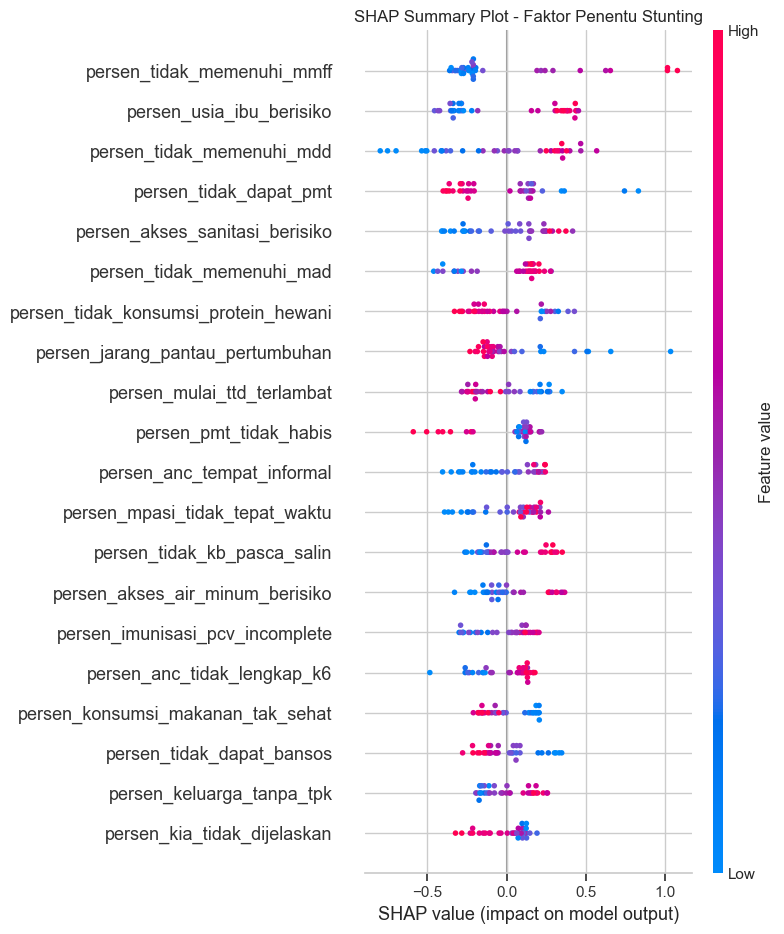
\includegraphics[width=0.75\textwidth]{figure/summary.png} 
    \caption{Arah dan Distribusi Dampak Fitur terhadap \textit{Stunting} (\textit{SHAP Summary Plot})}
    \label{fig:shap_summary}
\end{figure}

Berdasarkan Gambar \ref{fig:shap_summary}, terlihat bagaimana tiga variabel utama memberikan dorongan kenaikan terhadap tebakan prevalensi model. Pada variabel \texttt{persen\_tidak\_memenuhi\_mmff}, sebaran titik berwarna merah mendominasi area di sebelah kanan garis tegak (nol). Pola serupa juga ditemukan secara konsisten pada variabel persentase usia ibu berisiko dan kurangnya pemenuhan MDD. Sebaran ini membuktikan bahwa semakin tinggi persentase masalah kelengkapan gizi dan risiko usia ibu, maka prediksi kasus \textit{stunting} di suatu wilayah akan bertambah. Hasil distribusi warna yang sejalan dengan teori kesehatan ini menandakan bahwa algoritma telah berhasil memetakan pola sebab-akibat dengan akurat.

\subsubsection{Analisis Ketergantungan Fitur (\textit{Dependence Plot})}
Langkah terakhir dalam analisis skala global adalah menginterpretasikan distribusi nilai dari lima variabel dengan peringkat tertinggi. Pendekatan ini dilakukan menggunakan visualisasi \textit{SHAP Dependence Plot} untuk mencari titik batas perubahan pengaruh pada masing-masing indikator. Eksekusi sintaksis perulangan untuk menghasilkan kelima grafik tersebut secara berurutan ditunjukkan pada Kode 4.12. Visualisasi yang dihasilkan kemudian dirangkum secara komprehensif pada Gambar \ref{fig:grid_dependence_plot} dan dianalisis untuk melihat pada rentang angka berapa suatu variabel mulai merubah arah keputusan model. Penjelasan rincian dari setiap sub-grafik dijabarkan pada poin-poin di bawah ini.

\begin{lstlisting}[language=Python, caption={Visualisasi Ketergantungan Lima Fitur Teratas}, label={code:shap_dependence}, frame=single, basicstyle=\ttfamily\scriptsize, breaklines=true]
import matplotlib.pyplot as plt

# Daftar 5 fitur teratas berdasarkan SHAP
top5_features = [
    "persen_tidak_memenuhi_mmff",
    "persen_usia_ibu_berisiko",
    "persen_tidak_memenuhi_mdd",
    "persen_tidak_dapat_pmt",
    "persen_akses_sanitasi_berisiko"
]

# Visualisasi dependence plot per fitur
for feature in top5_features:
    plt.figure(figsize=(7, 5))
    shap.dependence_plot(
        feature, shap_values, X,
        interaction_index=None, 
        show=False
    )
    plt.title(f"SHAP Dependence Plot - {feature.replace('_', ' ').title()}", fontsize=13, pad=10)
    plt.xlabel("Nilai Fitur", fontsize=11)
    plt.ylabel("SHAP Value (Pengaruh terhadap Risiko Stunting)", fontsize=11)
    plt.tight_layout()
    plt.show()
\end{lstlisting}

\begin{figure}[htpb]
    \centering

    \begin{subfigure}[b]{0.48\textwidth}
        \centering
        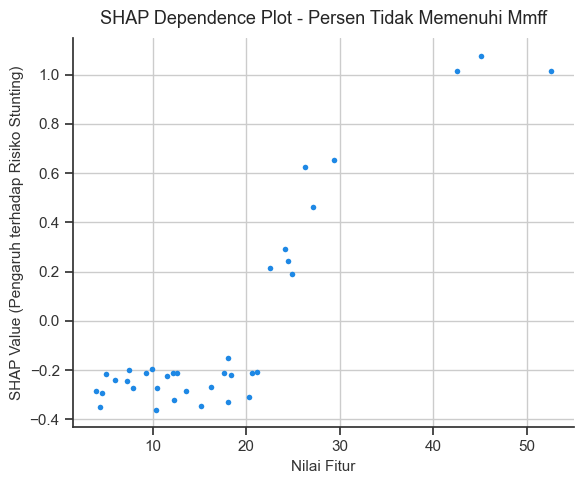
\includegraphics[width=\textwidth]{figure/dependence_mmff.png}
        \caption{Persen Tidak Memenuhi MMFF}
        \label{fig:dep_mmff}
    \end{subfigure}
    \hfill
    \begin{subfigure}[b]{0.48\textwidth}
        \centering
        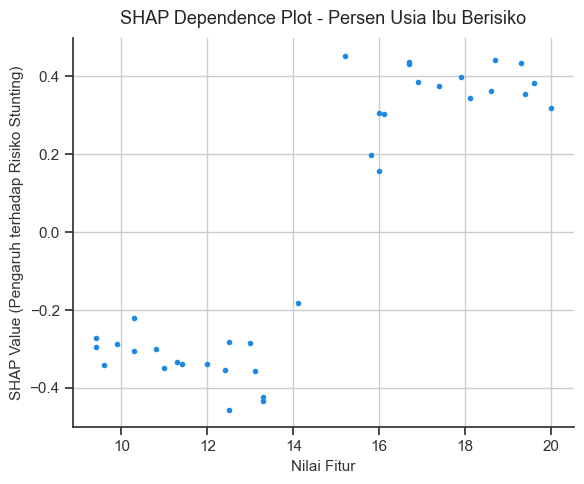
\includegraphics[width=\textwidth]{figure/dependence_usia_ibu.png}
        \caption{Persen Usia Ibu Berisiko}
        \label{fig:dep_usia_ibu}
    \end{subfigure}
    
    \vspace{0.3cm} 
    

    \begin{subfigure}[b]{0.48\textwidth}
        \centering
        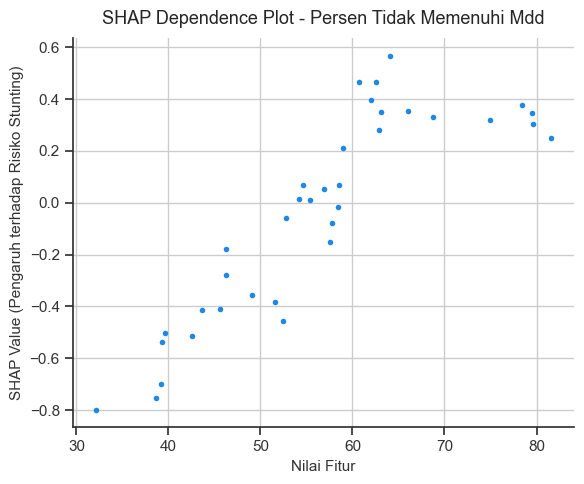
\includegraphics[width=\textwidth]{figure/dependence_mdd.png}
        \caption{Persen Tidak Memenuhi MDD}
        \label{fig:dep_mdd}
    \end{subfigure}
    \hfill
    \begin{subfigure}[b]{0.48\textwidth}
        \centering
        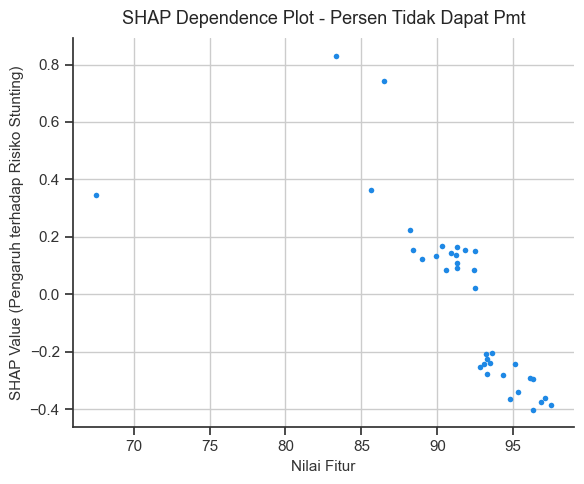
\includegraphics[width=\textwidth]{figure/dependence_pmt.png}
        \caption{Persen Tidak Dapat PMT}
        \label{fig:dep_pmt}
    \end{subfigure}
    
    \vspace{0.3cm} 
    
  
    \begin{subfigure}[b]{0.48\textwidth}
        \centering
        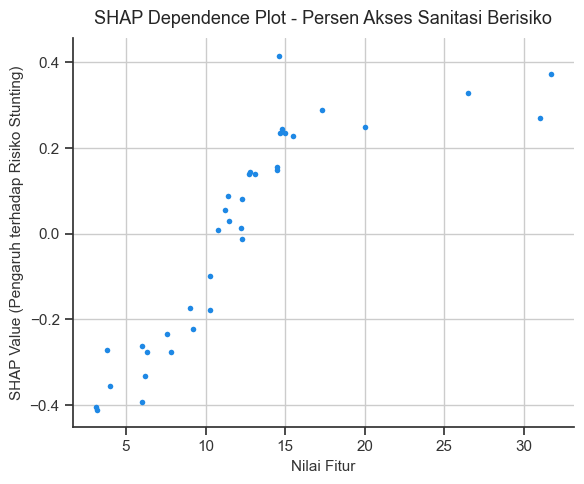
\includegraphics[width=\textwidth]{figure/dependence_sanitasi.png}
        \caption{Persen Akses Sanitasi Berisiko}
        \label{fig:dep_sanitasi}
    \end{subfigure}
    
    \caption{Visualisasi \textit{SHAP Dependence Plot} untuk Lima Determinan Teratas terhadap Probabilitas \textit{Stunting}}
    \label{fig:grid_dependence_plot}
\end{figure}

\newpage
\begin{enumerate}[listparindent=\parindent]
    \item Analisis Ketergantungan Variabel Tidak Memenuhi MMFF
    
    Gambar \ref{fig:dep_mmff} menampilkan grafik ketergantungan untuk fitur persentase tidak memenuhi MMFF. Berdasarkan sebaran titik pada visualisasi tersebut, nilai SHAP berada secara stabil di area negatif saat angka observasi berada di bawah 22\%. Namun, terdapat lonjakan drastis yang menyeberangi sumbu nol menuju area positif ketika persentase fitur melampaui ambang batas 22\% hingga 25\%. Semakin nilai persentase menjauhi batas tersebut ke arah kanan, dorongan terhadap risiko prediksi \textit{stunting} menjadi semakin tinggi secara signifikan. Pola ini membuktikan bahwa kurangnya asupan susu pada balita non-ASI memiliki batas toleransi maksimal di kisaran 22\% sebelum memicu lonjakan kasus.

    \indent Pola lonjakan risiko yang terlihat setelah melewati batas 22\% menunjukkan bahwa balita yang tidak lagi meminum ASI sangat rentan jika tidak diberikan asupan susu pengganti. Bagi anak yang sudah disapih, susu merupakan sumber utama kalsium dan protein yang perannya sangat penting untuk mendukung pertumbuhan tulang \cite{who2023complementary}. Perubahan drastis nilai SHAP menjadi positif setelah melewati batas toleransi ini menunjukkan terjadinya titik kegagalan pemenuhan gizi di suatu wilayah. Artinya, jika angka anak yang tidak mendapatkan susu sudah melebihi 22\%, makanan pengganti yang ada di masyarakat terbukti tidak mampu lagi menambal kekurangan nutrisi tersebut, yang pada akhirnya memicu lonjakan kasus \textit{stunting} \cite{beal2018review}. Temuan matematis dari algoritma ini secara langsung menegaskan bahwa asupan susu minimal adalah syarat wajib yang tidak bisa ditawar lagi bagi balita non-ASI.

    \item Analisis Ketergantungan Variabel Usia Ibu Berisiko
    
    Visualisasi ketergantungan untuk persentase usia ibu berisiko ditunjukkan pada Gambar \ref{fig:dep_usia_ibu}. Grafik ini memperlihatkan pola lonjakan nilai SHAP yang tegas ketika angka asli fitur melewati ambang batas 14\%. Pada rentang persentase di bawah 14\%, dampak yang diberikan cenderung bernilai negatif atau menekan angka prediksi. Sebaliknya, ketika persentase wilayah menyentuh angka 15\% ke atas, hasil tebakan langsung mendapat dorongan positif yang memicu kenaikan prediksi. Karakteristik ini mengindikasikan bahwa intervensi pencegahan kehamilan pada usia berisiko sebaiknya diupayakan agar tidak melampaui batas 14\%.

    \indent Peningkatan risiko yang terlihat saat melewati batas kritis ini sangat sejalan dengan kondisi fisik pada ibu hamil. Pada kehamilan di usia remaja, tubuh ibu yang sebenarnya masih dalam masa pertumbuhan terpaksa berebut gizi dengan janin yang dikandungnya \cite{Rahman2025}. Kondisi ini membuat penyaluran nutrisi ke janin menjadi terhambat, sehingga memperbesar kemungkinan bayi lahir dengan Berat Badan Lahir Rendah (BBLR). Sebaliknya, pada kehamilan di usia tua, penurunan fungsi organ tubuh ibu membuat penyaluran makanan ke kandungan menjadi tidak optimal, yang juga berisiko menghambat perkembangan janin \cite{Rahman2025}. Perubahan drastis nilai SHAP menjadi positif saat melewati batas 14\% membuktikan bahwa banyaknya bayi yang lahir dalam kondisi rentan ini akan langsung memperburuk angka \textit{stunting} di suatu wilayah. Temuan algoritma ini menegaskan pentingnya program edukasi dan perencanaan keluarga untuk menekan angka ibu hamil berisiko agar tetap berada di bawah ambang batas 14\%.

    \item Analisis Ketergantungan Variabel Tidak Memenuhi MDD
    
    Analisis ketergantungan untuk persentase balita tidak memenuhi MDD dapat diamati melalui sebaran titik pada Gambar \ref{fig:dep_mdd}. Indikator keberagaman makanan ini menunjukkan pola hubungan naik yang sejalan dengan peningkatan nilai aslinya. Titik kritis dari variabel ini terlihat secara jelas berada di sekitar angka 55\% ketika melewati sumbu nol. Semakin nilai persentase bergerak menjauhi ambang batas tersebut menuju angka 80\%, risiko prevalensi yang ditebak oleh model menjadi semakin tinggi. Pola distribusi ini menegaskan bahwa peningkatan masalah keberagaman asupan gizi secara proporsional akan menambah tinggi prediksi kasus di suatu wilayah.

    \indent Pola peningkatan risiko yang berbanding lurus dengan tingginya ketiadaan keberagaman pangan ini mengonfirmasi krusialnya variasi asupan pada masa pertumbuhan anak. Ketergantungan pada pola makan yang monoton, seperti hanya mengonsumsi sumber karbohidrat utama tanpa variasi protein dan sayuran, dapat menyebabkan tubuh balita kekurangan nutrisi esensial. Kurangnya asupan mineral dan vitamin penting seperti zink, zat besi, dan vitamin A secara langsung akan menghambat proses pembentukan tulang dan perkembangan fisik \cite{UNICEF2024_ChildFoodPoverty}. Lebih lanjut, perubahan drastis nilai perhitungan SHAP menjadi positif saat melewati ambang batas 55\% mengindikasikan tingginya kerentanan gizi di suatu wilayah. Hal ini menunjukkan bahwa apabila lebih dari separuh populasi balita tidak mendapatkan keberagaman makanan yang memadai, wilayah tersebut memiliki probabilitas kegagalan gizi komunal yang tinggi sehingga memicu lonjakan kasus \textit{stunting}. Temuan algoritma ini secara objektif memvalidasi urgensi pemenuhan keragaman konsumsi pangan sebagai strategi utama dalam menekan angka prevalensi.

    \item Analisis Ketergantungan Variabel Tidak Dapat PMT
    
    Gambar \ref{fig:dep_pmt} menjelaskan sebaran dampak dari variabel persentase sasaran yang tidak mendapatkan Pemberian Makanan Tambahan (PMT). Persebaran data pada visualisasi ini menunjukkan tarikan nilai SHAP yang tinggi saat angka asli fitur berada di bawah 85\%. Ketika persentase fitur mendekati rentang 90\% hingga 95\%, dampak variabel mulai melemah dan berpindah ke area nol hingga negatif. Karakteristik bentuk ini memperlihatkan dinamika kontribusi ketiadaan PMT yang tidak selalu lurus berbanding dengan prediksi hasil. Hasil pemetaan batas persentase ini memberikan informasi pendukung untuk mengevaluasi pemerataan bantuan PMT di wilayah observasi.

    \indent Pola non-linear pada grafik ini menunjukkan bahwa Pemberian Makanan Tambahan (PMT) pada dasarnya adalah bantuan pendamping, bukan pengganti makanan pokok sehari-hari \cite{kemenkes2023juknispmt}. Lonjakan risiko yang tinggi saat persentase balita tidak mendapat PMT berada di bawah 85\% mengindikasikan bahwa pada rentang tersebut, intervensi pemerintah masih dinilai penting sebagai langkah pemulihan awal untuk menutupi defisit gizi di tingkat rumah tangga. Namun, ketika angka ketiadaan bantuan mencapai skala yang sangat ekstrem (90\% hingga 95\%), pengaruh variabel ini di dalam model justru melemah. Kondisi ini terjadi karena wilayah dengan tingkat ketiadaan PMT setinggi itu umumnya memiliki masalah ketahanan pangan dasar yang jauh lebih parah. Pada situasi tersebut, tingginya angka \textit{stunting} lebih banyak dipengaruhi oleh kurangnya makanan harian (seperti keragaman lauk pauk dan asupan susu) serta buruknya kebersihan lingkungan, sehingga masalah ketiadaan PMT tidak lagi menjadi pemicu utamanya \cite{keats2021effective}. Temuan dari algoritma ini membuktikan bahwa pengaruh program PMT akan sangat bergantung pada pemerataan gizi dasar di wilayah tersebut.

    \item Analisis Ketergantungan Variabel Akses Sanitasi Berisiko
    
    Grafik ketergantungan kelima yang menjelaskan persentase akses sanitasi berisiko ditampilkan pada Gambar \ref{fig:dep_sanitasi}. Distribusi titik data pada sumbu vertikal memperlihatkan kecenderungan pergerakan naik secara berkelanjutan. Variabel sanitasi mulai memberikan sumbangsih positif terhadap peningkatan prediksi \textit{stunting} ketika angkanya melewati batas kritis 10\%. Pada persentase di bawah angka batas tersebut, nilai perhitungan SHAP berada di area negatif yang mendeskripsikan penurunan angka tebakan. Pemetaan dari model ini membuktikan bahwa wilayah observasi perlu menekan persentase ketiadaan akses sanitasi layak di bawah batas 10\%.

    \indent Peningkatan risiko \textit{stunting} yang berbanding lurus dengan memburuknya fasilitas sanitasi sangat berkaitan erat dengan paparan bakteri dari lingkungan. Secara kajian kesehatan masyarakat, buruknya akses sanitasi akan mempermudah penularan kuman penyakit yang memicu infeksi pencernaan berulang pada anak. Gangguan pencernaan kronis ini mengakibatkan usus tidak mampu menyerap nutrisi dari makanan secara maksimal, padahal gizi tersebut sangat dibutuhkan untuk mendukung pertumbuhan fisik balita \cite{kemenkes2022tatalaksana}. Selanjutnya, kemunculan ambang batas kritis pada angka 10\% mengindikasikan pentingnya menjaga kebersihan lingkungan secara komunal. Apabila jumlah rumah tangga tanpa sanitasi layak di suatu wilayah melampaui batas toleransi tersebut, pencemaran bakteri pada sumber air dan tanah akan menjadi terlalu masif sehingga memicu keadaan inflamasi kronis pada tubuh balita, di mana sistem kekebalan tubuh bekerja terlalu keras tanpa henti untuk melawan infeksi \cite{torlesse2016determinants}. Temuan ambang batas dari algoritma ini membuktikan bahwa penyediaan infrastruktur sanitasi yang bersih adalah syarat wajib agar makanan bergizi yang diberikan dapat diserap secara optimal oleh tubuh anak.

\end{enumerate}

\subsection{Interpretasi Lokal (\textit{Local Explanation})}
Analisis skala lokal bertujuan untuk menjelaskan proses pengambilan keputusan algoritma pada satu observasi data yang spesifik. Berbeda dengan pendekatan global yang memetakan tren secara keseluruhan, tahapan ini berfokus pada faktor-faktor pendorong hasil tebakan pada kasus tunggal. Pendekatan ini berguna untuk memahami alasan di balik tingginya atau rendahnya prediksi prevalensi \textit{stunting} pada sampel wilayah tertentu. Visualisasi pada tahap ini akan menampilkan bagaimana masing-masing variabel berkontribusi secara rinci dalam menambah atau menekan nilai dasar model. Hasil interpretasi dari observasi tunggal ini kemudian dapat diuraikan sebagai rujukan evaluasi khusus bagi wilayah yang bersangkutan.

\subsubsection{Kriteria Pemilihan Sampel Wilayah}
Sebelum melakukan ekstraksi visualisasi \textit{Local Explanation}, tahap penentuan sampel observasi perlu dilakukan agar analisis lebih terarah. Pemilihan sampel provinsi pada penelitian ini menggunakan teknik \textit{purposive sampling} yang didasarkan pada enam kriteria kondisi demografis dan tingkat prevalensi. Keenam sampel tersebut dirancang untuk merepresentasikan berbagai variasi keadaan yang memengaruhi hasil tebakan algoritma secara spesifik. Melalui variasi observasi ini, model diharapkan mampu menunjukkan perbedaan pola pengambilan keputusan pada setiap kasus secara transparan.

Kriteria pertama difokuskan pada kedekatan geografis dan keterwakilan regional Pulau Sumatera sebagai lokasi institusi tempat penelitian ini dilakukan. Provinsi Lampung dipilih sebagai representasi wilayah utama karena merupakan domisili pelaksanaan penelitian di Institut Teknologi Sumatera. Selain Lampung, Provinsi Aceh dan Sumatera Utara turut dipilih untuk mewakili karakteristik regional Sumatera masing-masing, yakni sebagai wilayah dengan angka prevalensi \textit{stunting} tertinggi dan wilayah dengan populasi terpadat di pulau tersebut yang mencapai lebih dari 15,4 juta jiwa \cite{bps2024statistik}. Peninjauan khusus pada ketiga provinsi ini bertujuan untuk memberikan kontribusi akademis yang relevan terhadap identifikasi dan penanganan masalah kesehatan di wilayah Sumatera.

Kriteria selanjutnya mencakup pemilihan provinsi yang memegang rekor ekstrem pada skala nasional untuk melihat respons model terhadap kondisi data yang kontras. Analisis pada wilayah dengan prevalensi tertinggi secara nasional, yakni Provinsi Nusa Tenggara Timur (NTT) dengan angka \textit{stunting} mencapai 37,0\%, bertujuan untuk menemukan pemicu utama krisis gizi. Sementara itu, Provinsi Bali yang berhasil menekan prevalensi hingga menyentuh angka terendah secara nasional sebesar 8,7\% berfungsi sebagai pembanding keberhasilan intervensi. Provinsi Jawa Barat sebagai wilayah dengan populasi penduduk terpadat di tingkat nasional yang menembus lebih dari 50,4 juta jiwa \cite{bps2024statistik} juga disertakan untuk meninjau dampak persaingan akses sumber daya terhadap hasil prediksi. Penggabungan sampel regional dan nasional ini ditujukan agar visualisasi skala lokal dapat memberikan gambaran yang menyeluruh mengenai kinerja model \textit{machine learning}.

\subsubsection{Analisis Skala Lokal (\textit{Waterfall Plot})}
Tahapan interpretasi skala lokal dilakukan dengan mengeksekusi visualisasi \textit{SHAP Waterfall Plot} untuk menginterpretasikan data observasi secara spesifik. Proses komputasi ini bertujuan untuk menguraikan kontribusi masing-masing variabel dalam mendorong atau menekan nilai rata-rata dasar prediksi model (\textit{base value}) yang berada pada angka 22,375. \textit{Base value} diperoleh dari rata-rata prediksi model terhadap seluruh data latih. Implementasi ekstraksi grafik untuk seluruh provinsi secara otomatis beserta proses penyimpanannya ditunjukkan pada Kode 4.13. Berdasarkan hasil pemrosesan tersebut, analisis mendalam difokuskan pada enam provinsi yang telah ditetapkan melalui kriteria \textit{purposive sampling} sebelumnya. Rincian penjabaran kontribusi fitur penentu \textit{stunting} untuk keenam sampel wilayah tersebut diuraikan sebagai berikut.

\begin{lstlisting}[language=Python, caption={Visualisasi dan Ekstraksi Waterfall Plot Seluruh Provinsi}, label={code:waterfall_all}, frame=single, basicstyle=\ttfamily\scriptsize, breaklines=true]
# SHAP waterfall plot value for a specific province
explainer = shap.TreeExplainer(model_final)
shap_values = explainer(X)

nama_folder = "hasil_waterfall_stunting"

if not os.path.exists(nama_folder):
    os.makedirs(nama_folder)
    print(f"Folder '{nama_folder}' berhasil dibuat!")

daftar_provinsi = plot_data_clean['Provinsi'].tolist()

for i in range(len(shap_values)):
    prov_name = daftar_provinsi[i]
    file_name = f"waterfall_{prov_name.replace(' ', '_')}.png"
    path_simpan = os.path.join(nama_folder, file_name)
    
    plt.figure(figsize=(10, 7))
    shap.plots.waterfall(shap_values[i], show=False)
    plt.suptitle(f"Kontribusi Fitur terhadap Prediksi Stunting - Provinsi {prov_name}", 
                 fontsize=14, y=1.05, fontweight='bold')
    
    plt.figtext(
        0.5, -0.02,
        "Merah = menaikkan risiko stunting | Biru = menurunkan risiko stunting",
        ha='center', fontsize=11, color='gray', style='italic'
    )
    
    plt.tight_layout()
    plt.savefig(path_simpan, dpi=300, bbox_inches='tight')
    plt.show()
    plt.close()

print(f"\nSelesai! Semua gambar sudah tersimpan di folder: {nama_folder}")
\end{lstlisting}

\begin{enumerate}
    \item Provinsi Lampung (Representasi Domisili Institusi)
    \begin{figure}[H]
        \centering
        
\includegraphics[width=0.85\textwidth]{figure/waterfall_Lampung.png} 
        \caption{\textit{Waterfall Plot} Prediksi \textit{Stunting} Provinsi Lampung}
        \label{fig:wf_lampung}
    \end{figure}

    Visualisasi pada Gambar \ref{fig:wf_lampung} menampilkan distribusi pengaruh fitur untuk Provinsi Lampung dengan hasil tebakan akhir sebesar 18,63. Penurunan dari nilai dasar ini didominasi secara penuh oleh kontribusi negatif (warna biru) dari mayoritas indikator kesehatan. Faktor sasaran balita tidak dapat PMT, risiko akses sanitasi, dan persentase usia ibu berisiko menjadi variabel teratas yang menekan angka prevalensi. Tarikan searah tanpa adanya perlawanan balok merah ini mengindikasikan bahwa fasilitas kesehatan dasar di wilayah Lampung secara umum sudah cukup menekan potensi lonjakan kasus \textit{stunting}.

    \item Provinsi Aceh (Prevalensi Tertinggi Regional Sumatera)
    \begin{figure}[H]
        \centering
        
\includegraphics[width=0.85\textwidth]{figure/waterfall_Aceh.png} 
        \caption{\textit{Waterfall Plot} Prediksi \textit{Stunting} Provinsi Aceh}
        \label{fig:wf_aceh}
    \end{figure}

    Observasi skala lokal untuk Provinsi Aceh memproyeksikan tebakan model yang melonjak tinggi menuju angka 26,301. Berdasarkan Gambar \ref{fig:wf_aceh}, peningkatan ini didorong kuat oleh sekumpulan balok merah yang mempresentasikan nilai positif terhadap prediksi risiko. Variabel kurangnya pemenuhan MMFF dan jarangnya pemantauan pertumbuhan balita menjadi pemicu utama dengan kontribusi dorongan terbesar. Tingginya tumpukan fitur pembawa risiko ini merepresentasikan akar permasalahan gizi yang memerlukan intervensi segera di wilayah tersebut.

    \item Provinsi Sumatera Utara (Populasi Terpadat Regional Sumatera)
    \begin{figure}[H]
        \centering
        
\includegraphics[width=0.85\textwidth]{figure/waterfall_Sumatera_Utara.png} 
        \caption{\textit{Waterfall Plot} Prediksi \textit{Stunting} Provinsi Sumatera Utara}
        \label{fig:wf_sumut}
    \end{figure}

    Dinamika kontribusi yang saling mengimbangi terlihat pada grafik distribusi Provinsi Sumatera Utara di Gambar \ref{fig:wf_sumut}. Prediksi model untuk wilayah ini berakhir pada angka 22,501, yang sangat mendekati nilai rata-rata dasar prediksi nasional. Penekanan risiko oleh variabel pemenuhan MAD dan usia ibu berisiko mendapat perlawanan dari dorongan risiko akibat indikator tidak KB pasca salin dan imunisasi PCV yang tidak lengkap. Keseimbangan antara balok penekan dan pendorong ini menggambarkan kompleksitas tantangan fasilitas kesehatan di wilayah dengan padat penduduk.

    \item Provinsi Nusa Tenggara Timur (Prevalensi Tertinggi Nasional)
    \begin{figure}[H]
        \centering
        
\includegraphics[width=0.85\textwidth]{figure/waterfall_Nusa_Tenggara_Timur.png} 
        \caption{\textit{Waterfall Plot} Prediksi \textit{Stunting} Provinsi Nusa Tenggara Timur}
        \label{fig:wf_ntt}
    \end{figure}

    Gambar \ref{fig:wf_ntt} menjelaskan secara ekstrem pemicu di balik rekor prevalensi tertinggi secara nasional di Provinsi Nusa Tenggara Timur. Model menghasilkan tebakan akhir yang sangat tinggi di angka 33,815 dengan grafik yang didominasi oleh pergerakan balok merah secara masif. Kurangnya asupan susu (MMFF) dan minimnya pemantauan pertumbuhan memberikan sumbangsih penambahan risiko terbesar, masing-masing sebesar +1,0. Identifikasi tumpukan pendorong arah positif ini menegaskan keparahan krisis kelengkapan gizi dasar dan fasilitas pemantauan anak di wilayah tersebut.

    \newpage
    \item Provinsi Bali (Prevalensi Terendah Nasional)
    \begin{figure}[H]
        \centering
        
\includegraphics[width=0.85\textwidth]{figure/waterfall_Bali.png} 
        \caption{\textit{Waterfall Plot} Prediksi \textit{Stunting} Provinsi Bali}
        \label{fig:wf_bali}
    \end{figure}

    Sebagai representasi wilayah dengan angka kasus terendah, \textit{Waterfall Plot} Provinsi Bali pada Gambar \ref{fig:wf_bali} memperlihatkan pola sapuan biru yang sempurna. Prediksi akhir wilayah ini ditekan secara drastis hingga mencapai angka 12,565 tanpa adanya satu pun fitur utama yang memberi dorongan risiko. Keberagaman asupan makanan (MDD) dan efektivitas PMT menjadi indikator terkuat yang mengurangkan nilai prediksi dasar. Ketiadaan balok merah pada grafik ini mengonfirmasi kualitas standar keunggulan kesehatan ibu dan anak yang sangat baik di wilayah Bali.

    \newpage
    \item Provinsi Jawa Barat (Populasi Terpadat Nasional)
    \begin{figure}[H]
        \centering
        
\includegraphics[width=0.85\textwidth]{figure/waterfall_Jawa_Barat.png} 
        \caption{\textit{Waterfall Plot} Prediksi \textit{Stunting} Provinsi Jawa Barat}
        \label{fig:wf_jabar}
    \end{figure}
    
    Analisis visualisasi untuk provinsi dengan populasi terpadat, yaitu Jawa Barat, dapat diamati melalui Gambar \ref{fig:wf_jabar}. Meskipun memiliki tekanan persaingan akses yang tinggi, model memprediksi penurunan angka prevalensi menuju nilai 17,755. Penurunan ini didorong secara konsisten oleh efektivitas program PMT dan kecukupan keberagaman pangan (MDD). Terdapat satu variabel yang memberikan dorongan risiko kecil, yakni masalah akses sanitasi berisiko, yang merupakan dampak logis dari kepadatan permukiman penduduk di wilayah tersebut.
\end{enumerate}